\usepackage[utf8]{inputenc}
\usepackage[T1]{fontenc}
\usepackage[english]{babel}
\usepackage{graphicx}
\usepackage[a4paper,
            left=25mm,
            right=20mm,
            top=15mm,       % This is what you want - 15mm from top
            bottom=25mm,
            headheight=15pt,
            headsep=15pt
           ]{geometry}
\usepackage{xcolor}
\usepackage{fancyhdr}
\usepackage{caption}
\usepackage{tocloft}
\usepackage{url}
\geometry{top=2.5cm, bottom=2.5cm, left=2.5cm, right=2.5cm}
\usepackage{titlesec}
\usepackage{tabularx}
\usepackage[dvipsnames,svgnames,x11names,table]{xcolor}
\usepackage{array}
\usepackage{booktabs}
\usepackage{tabularray}
\usepackage{multicol}
\UseTblrLibrary{booktabs}
\geometry{margin=1.5cm}
\usepackage[autostyle]{csquotes}
\usepackage[backend=biber, style=ieee]{biblatex}
\usepackage{listings}
\addbibresource{Netnography.bib}
\pagestyle{fancy}
\raggedbottom
\hbadness=10000
\vbadness=10000
\fancyhf{}
\fancyhead[R]{\thepage}
% Display fixed text on inside corners (Left Odd, Right Even)
\fancyhead[L]{\textit{\nouppercase{\leftmark}}}   % Chapter on all left headers
% Format main title "Dédicaces"

% Custom section command for names
\newcommand{\dedicationsection}[1]{%
  \vspace{1.5em}
  \noindent{\Large\bfseries #1}\par\medskip
}
% Line thickness
\renewcommand{\headrulewidth}{0.4pt}
\renewcommand{\footrulewidth}{0pt}
% Enhanced figure and table captions
\captionsetup{font=small,labelfont=bf,format=hang,margin=10pt}
% Logo definitions
\newcommand{\logoISTIC}{
\includegraphics[height=2.5cm]{Images/logo_ISTIC.png}}
\newcommand{\logoMinistereISTIC}{
\includegraphics[height=3.4cm]{Images/logo_ministere_ISTIC_text.png}}
\newcommand{\logoCarthage}{
\includegraphics[height=2.5cm]{Images/logo_carthage_universit.png}}
\newcommand{\logoTELECOM}{
\includegraphics[height=2.2cm]{Images/logo_telecom.png}}
\newcommand{\Telecom}{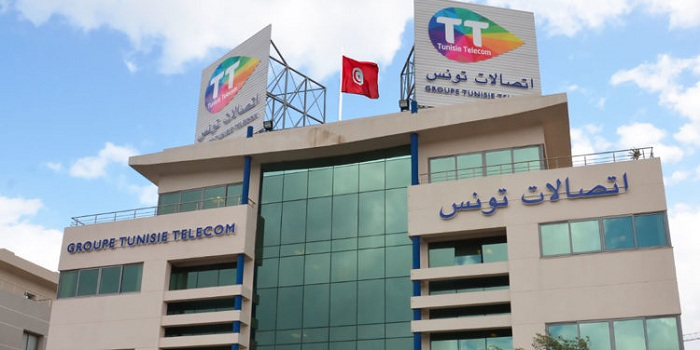
\includegraphics[height=7.5cm]{Images/telecom.jpg}}
\newcommand{\OrgTelecom}{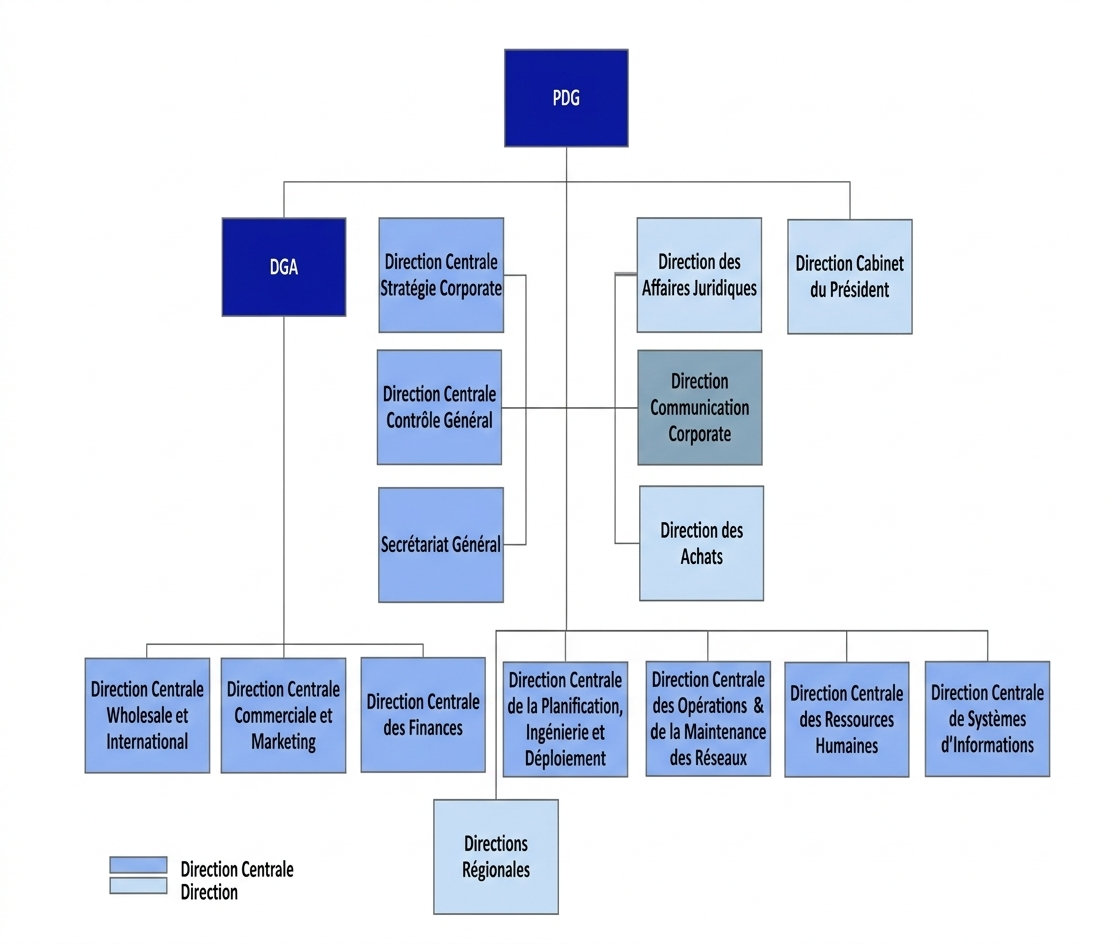
\includegraphics[width=\textwidth,height=9.5cm]{Images/organchartTelecom.png}}
\newcommand{\PratnerGrid}{
\includegraphics[width=\textwidth,height=4.5cm]{Images/pranter_grid.png}}
\newcommand{\agiletimeline}{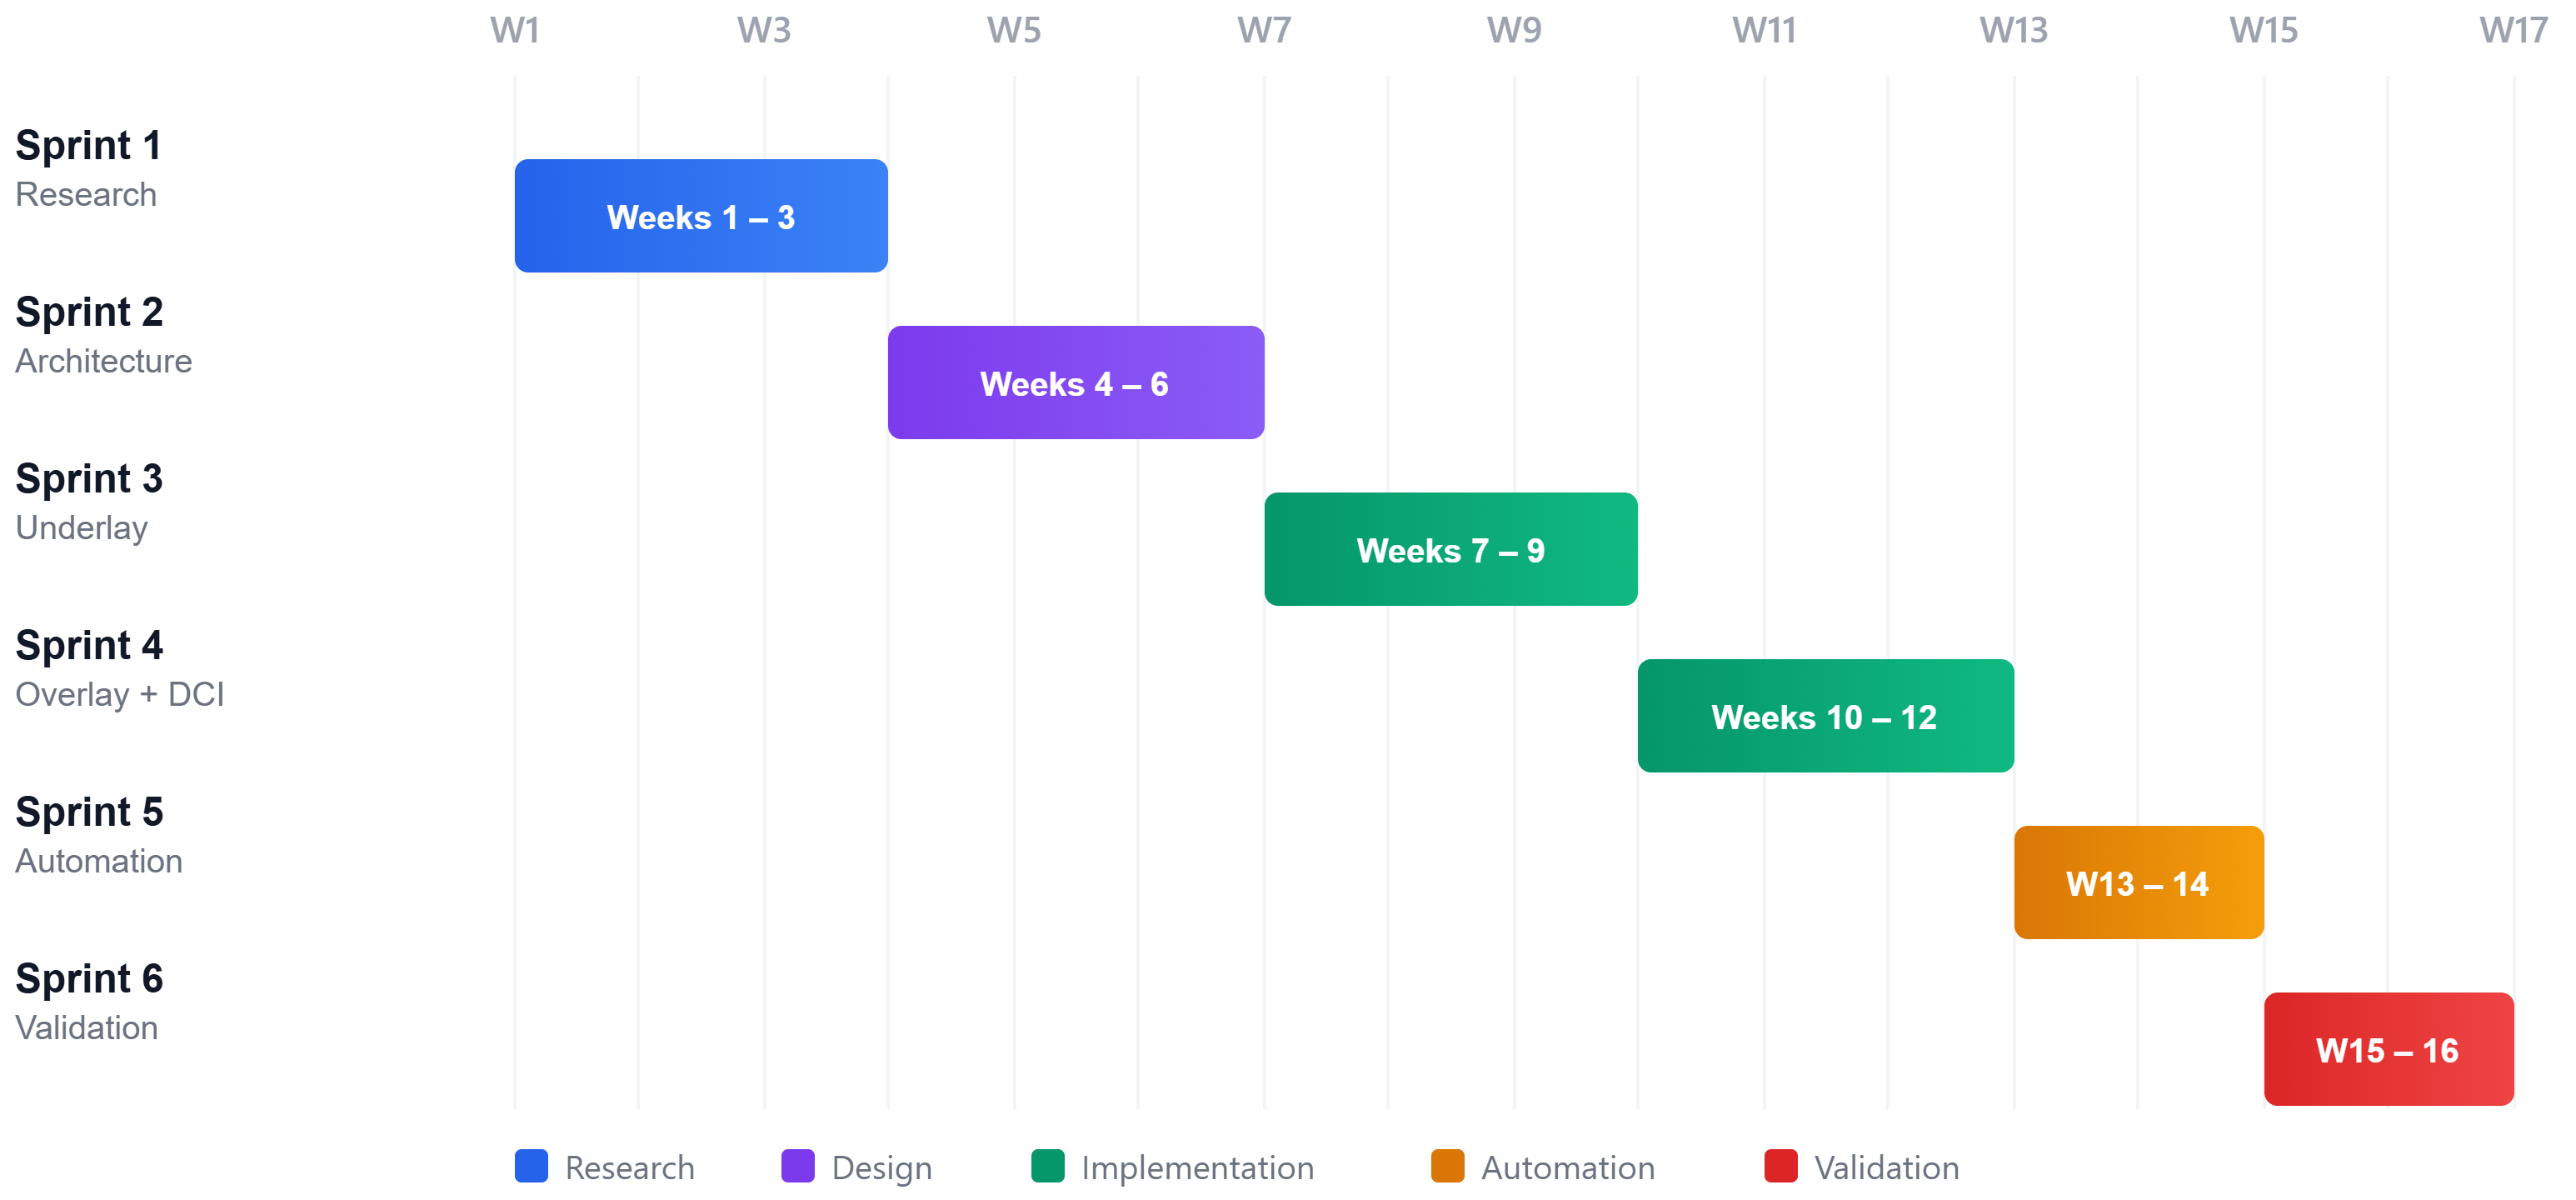
\includegraphics[width=\textwidth,height=6.85cm]{Images/agiletimeline.png}}
\newcommand{\ComputingEvolutionEra}{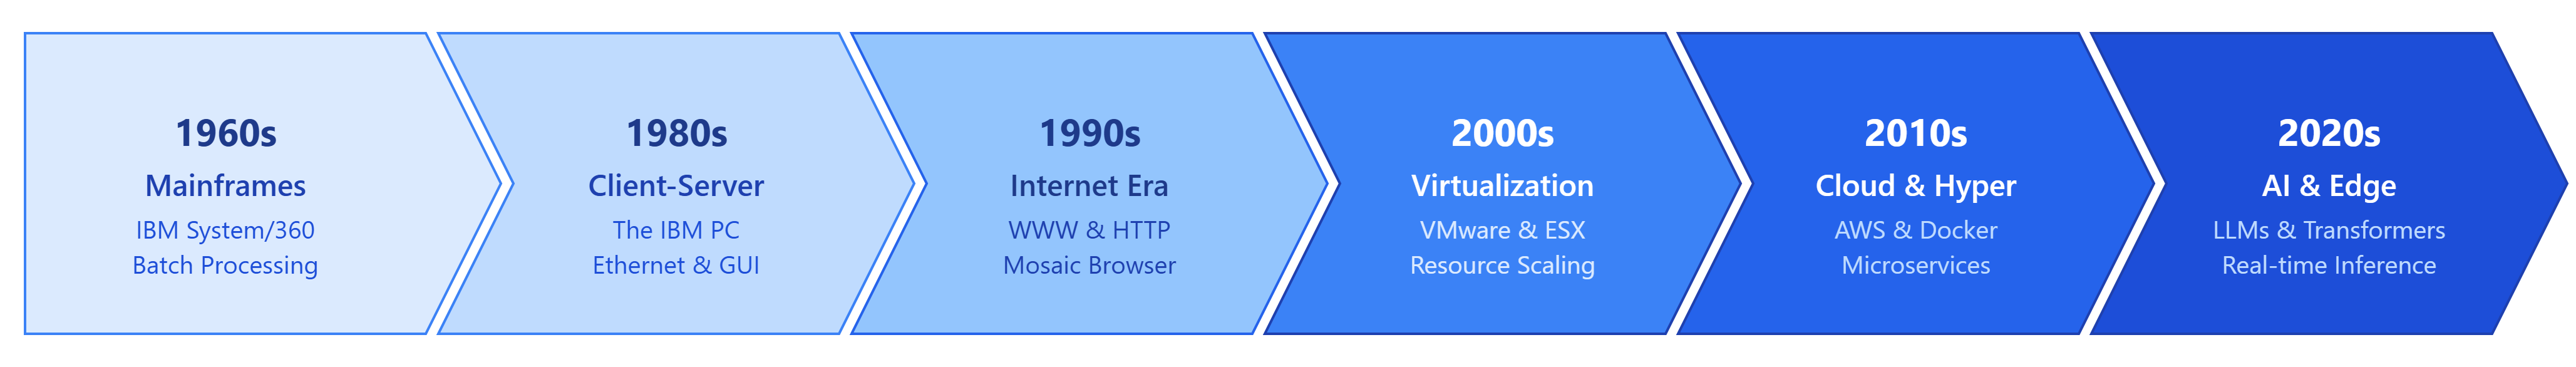
\includegraphics[width=\textwidth,height=3.1cm]{Images/ComputingEvolutionEra.png}}
\newcommand{\Architecturethreetier}{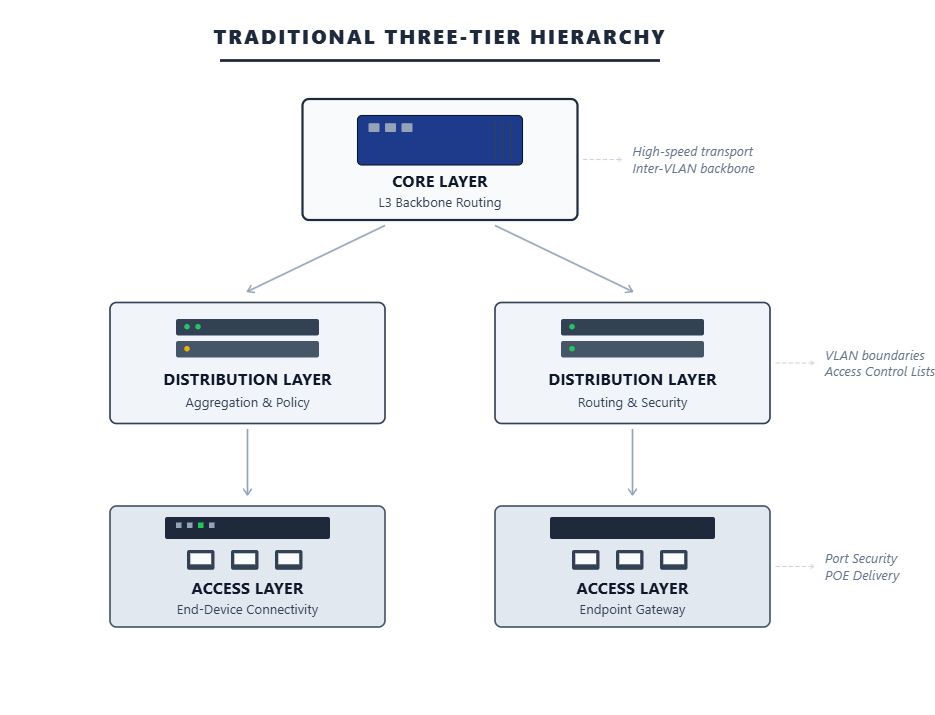
\includegraphics[width=0.8\textwidth,height=8.1cm]{Images/architec_3tier.png}}
\newcommand{\SDNarchitecture}{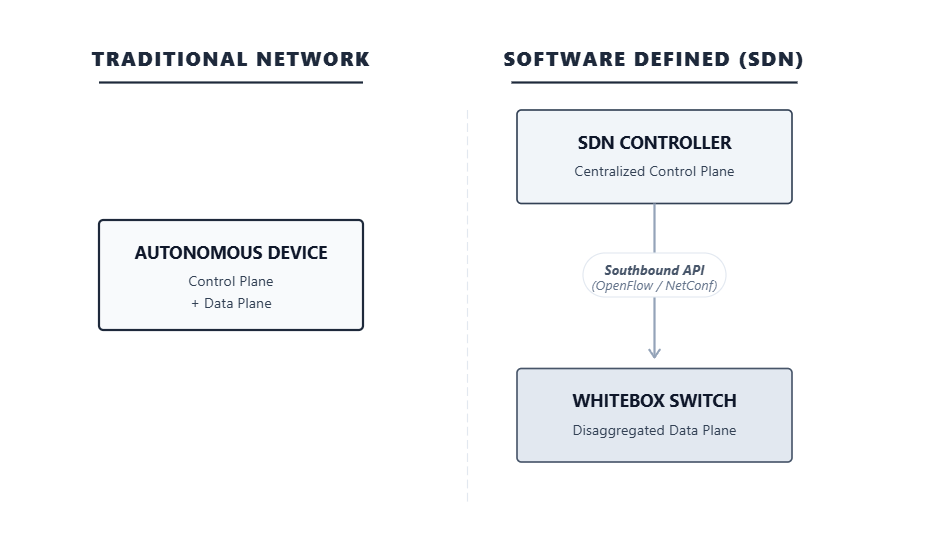
\includegraphics[width=0.8\textwidth,height=6.5cm]{Images/SDN_architecture.png}}
\newcommand{\NFVtimeline}{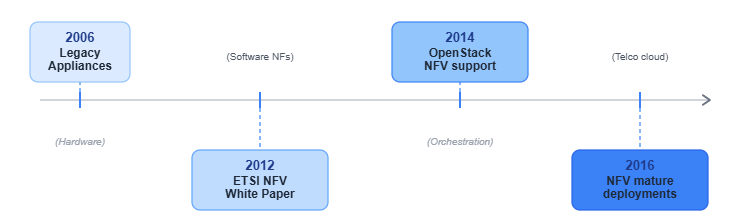
\includegraphics[height=5.1cm]{Images/NFV_timeline.png}}
\newcommand{\SpineLeafDiagram}{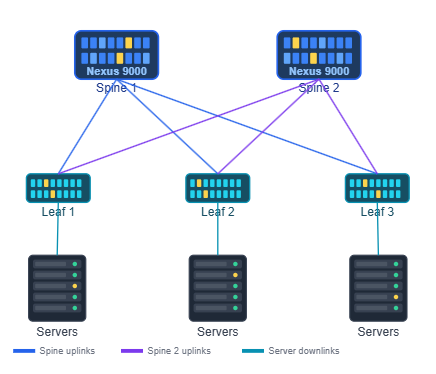
\includegraphics[width=0.9\textwidth,height=5.5cm]{Images/Spine-Leafdiag.png}}
\newcommand{\underoverlay}{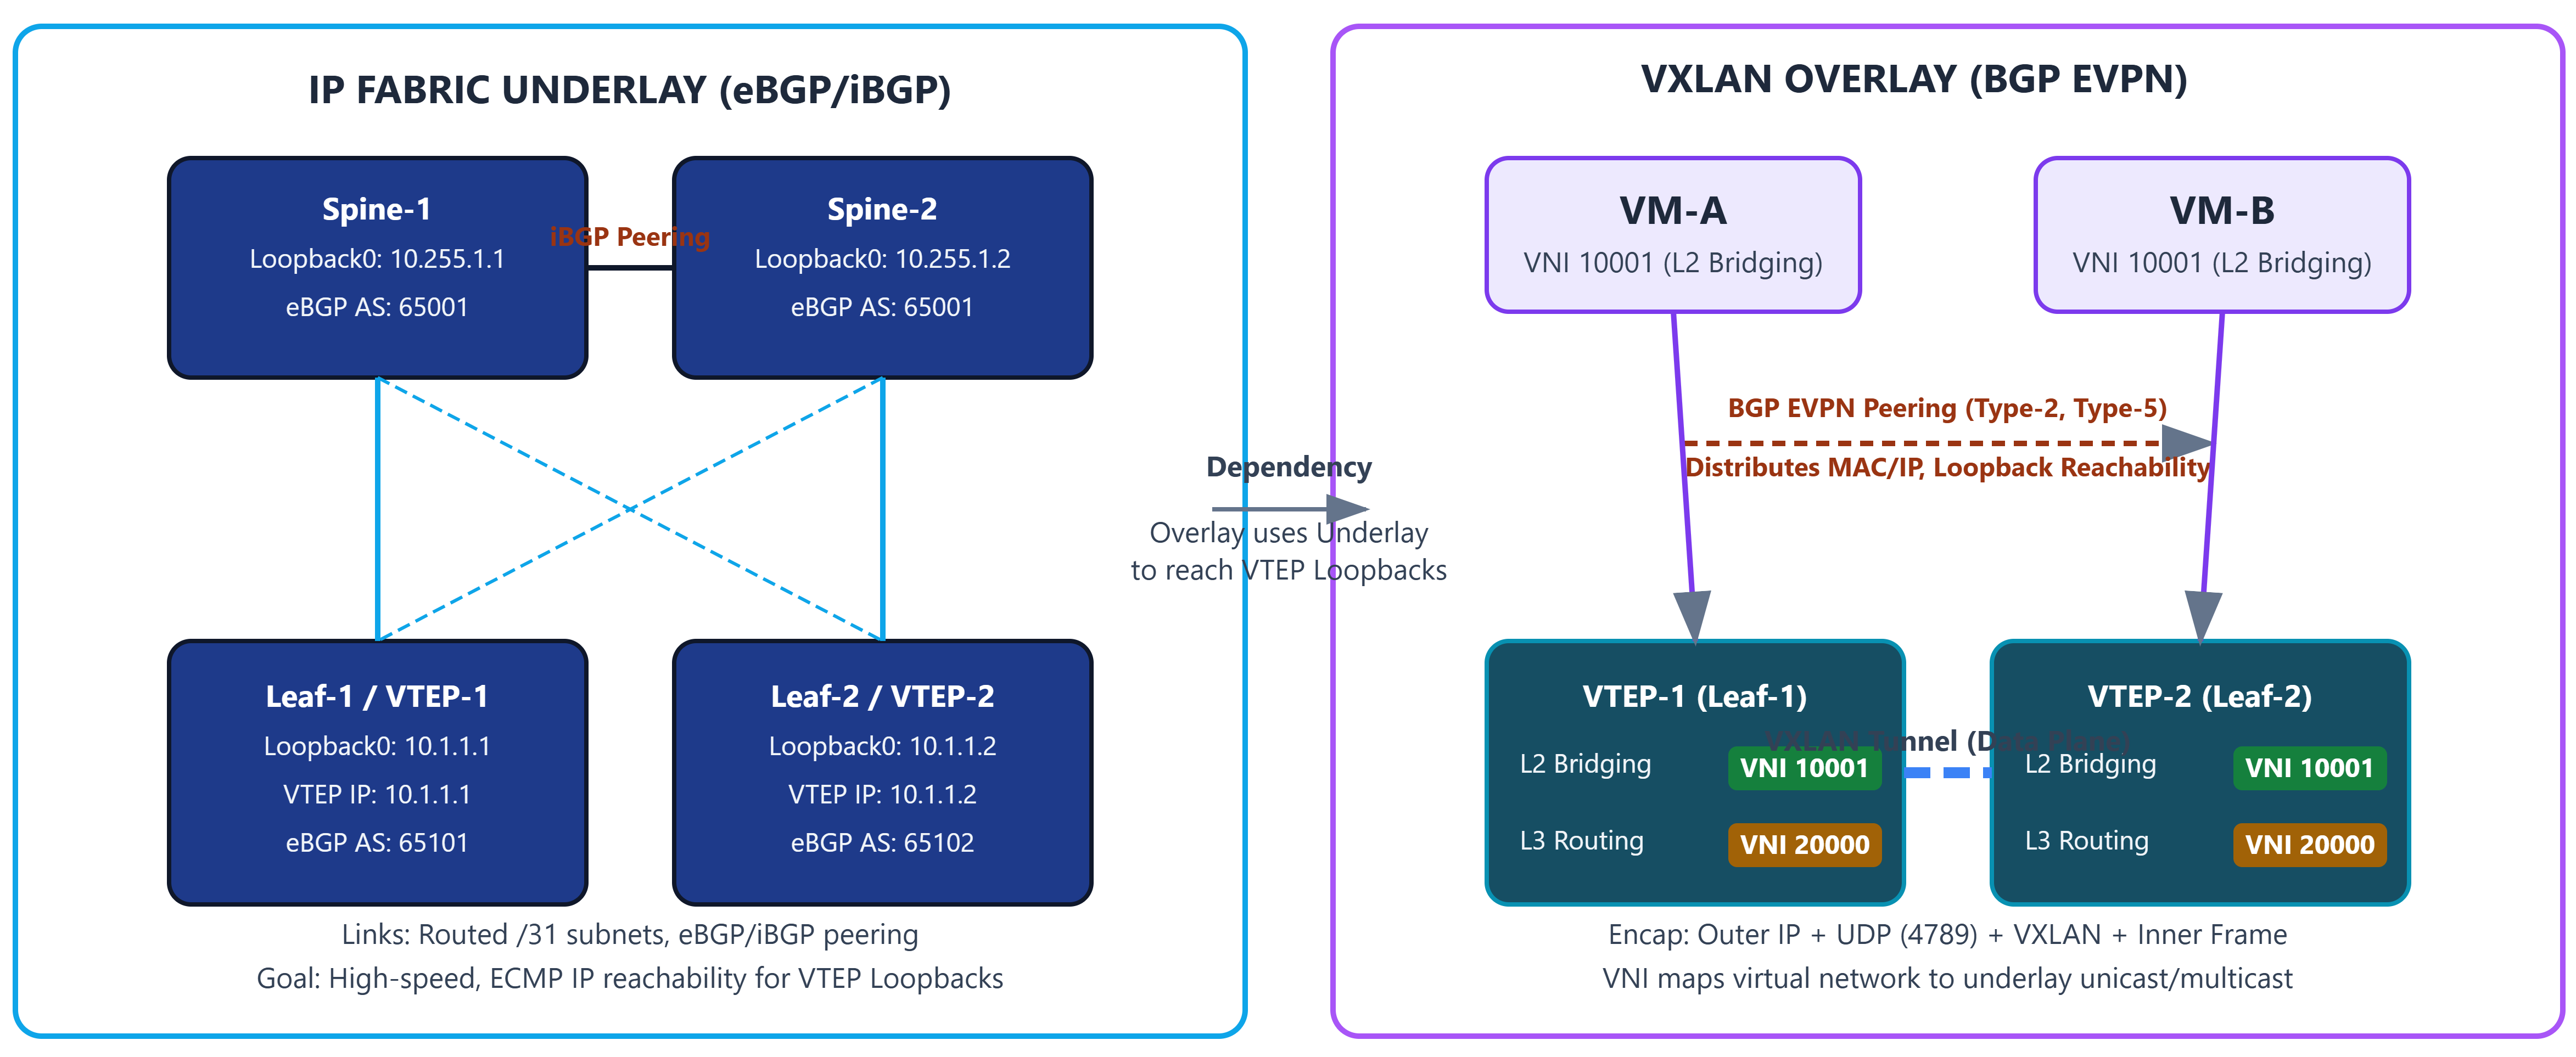
\includegraphics[width=\textwidth,height=7.5cm]{Images/Diagunderlayoverlay.png}}
\newcommand{\overlayunderlay}{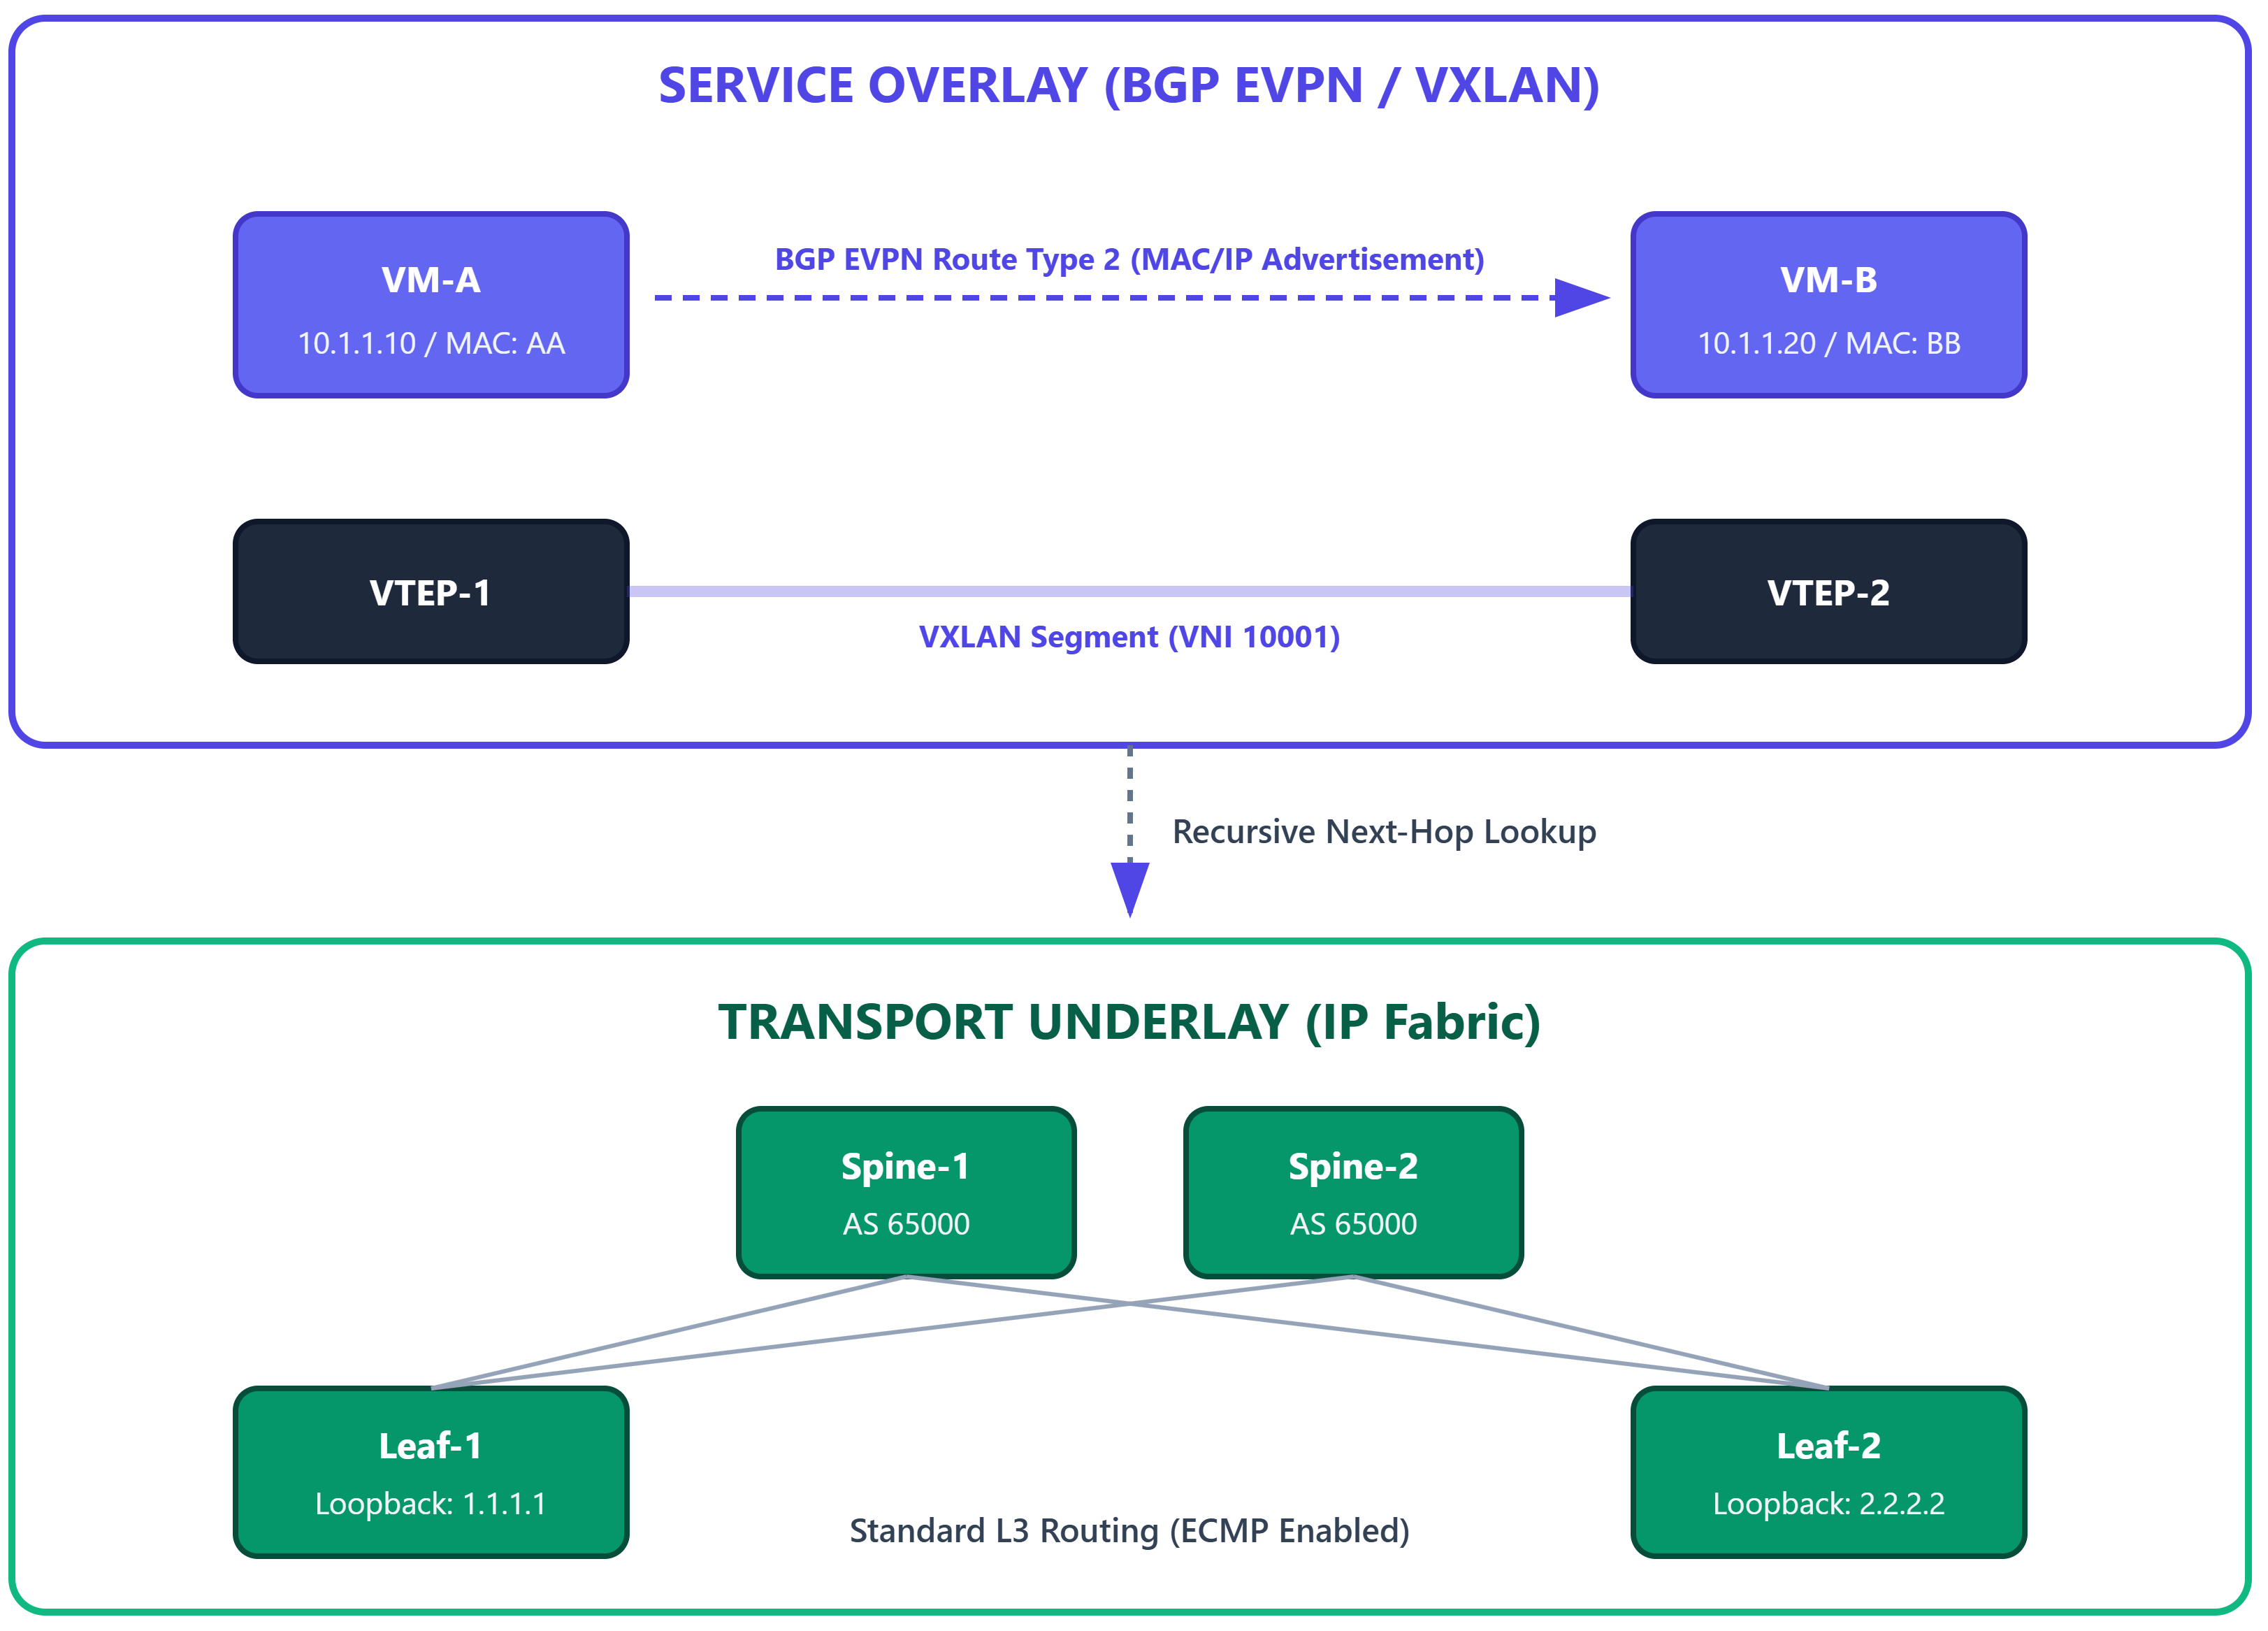
\includegraphics[width=\textwidth,height=9cm]{Images/Diagoverlayunderlaysplit.png}}
\newcommand{\TCPvsOSI}{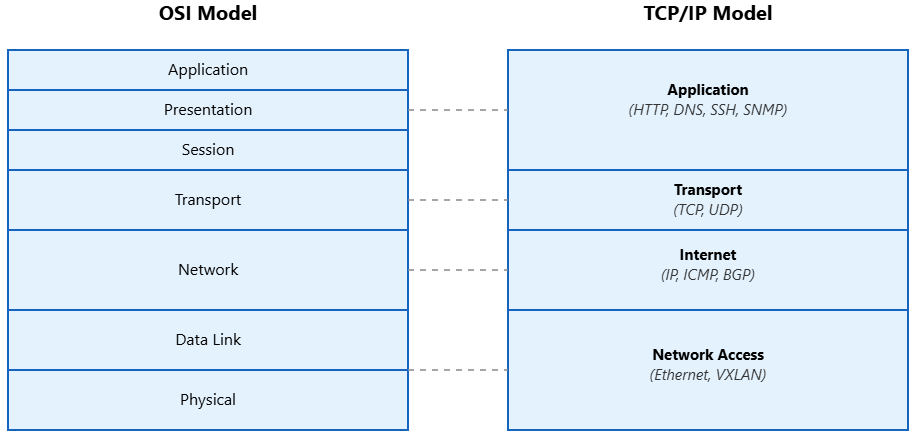
\includegraphics[width=\textwidth,height=5.5cm]{Images/TCPvsIOS.png}}
\newcommand{\networkautomation}{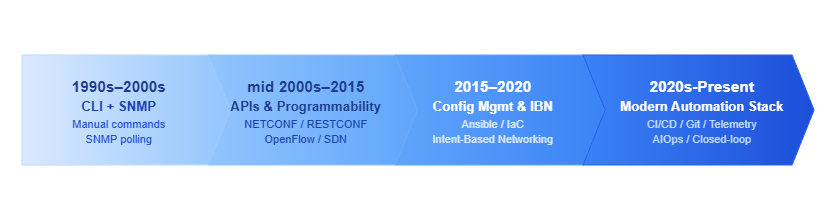
\includegraphics[width=1.0\textwidth,height=2.5cm]{Images/NetworkAutomationTimeline.png}}
\newcommand{\BGPhistory}{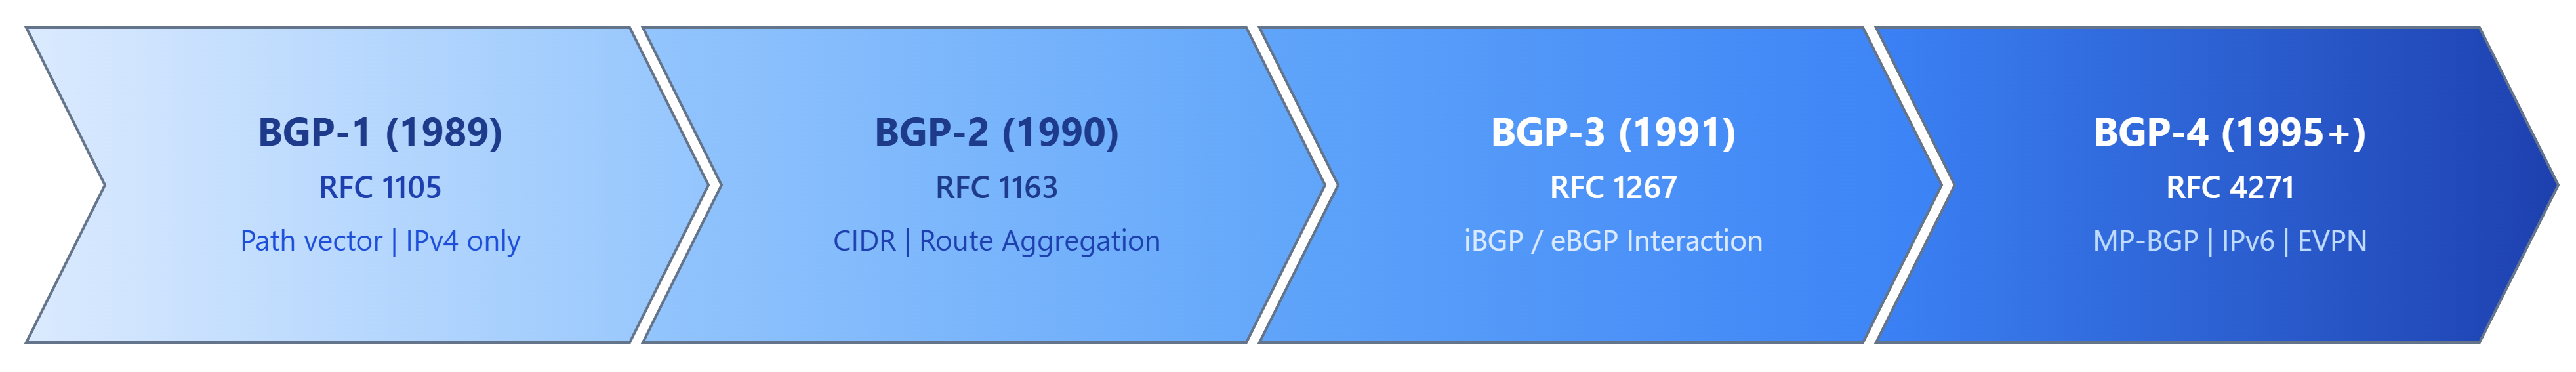
\includegraphics[width=1.0\textwidth,height=2.5cm]{Images/Bgphstory.png}}
\newcommand{\BGPMFS}{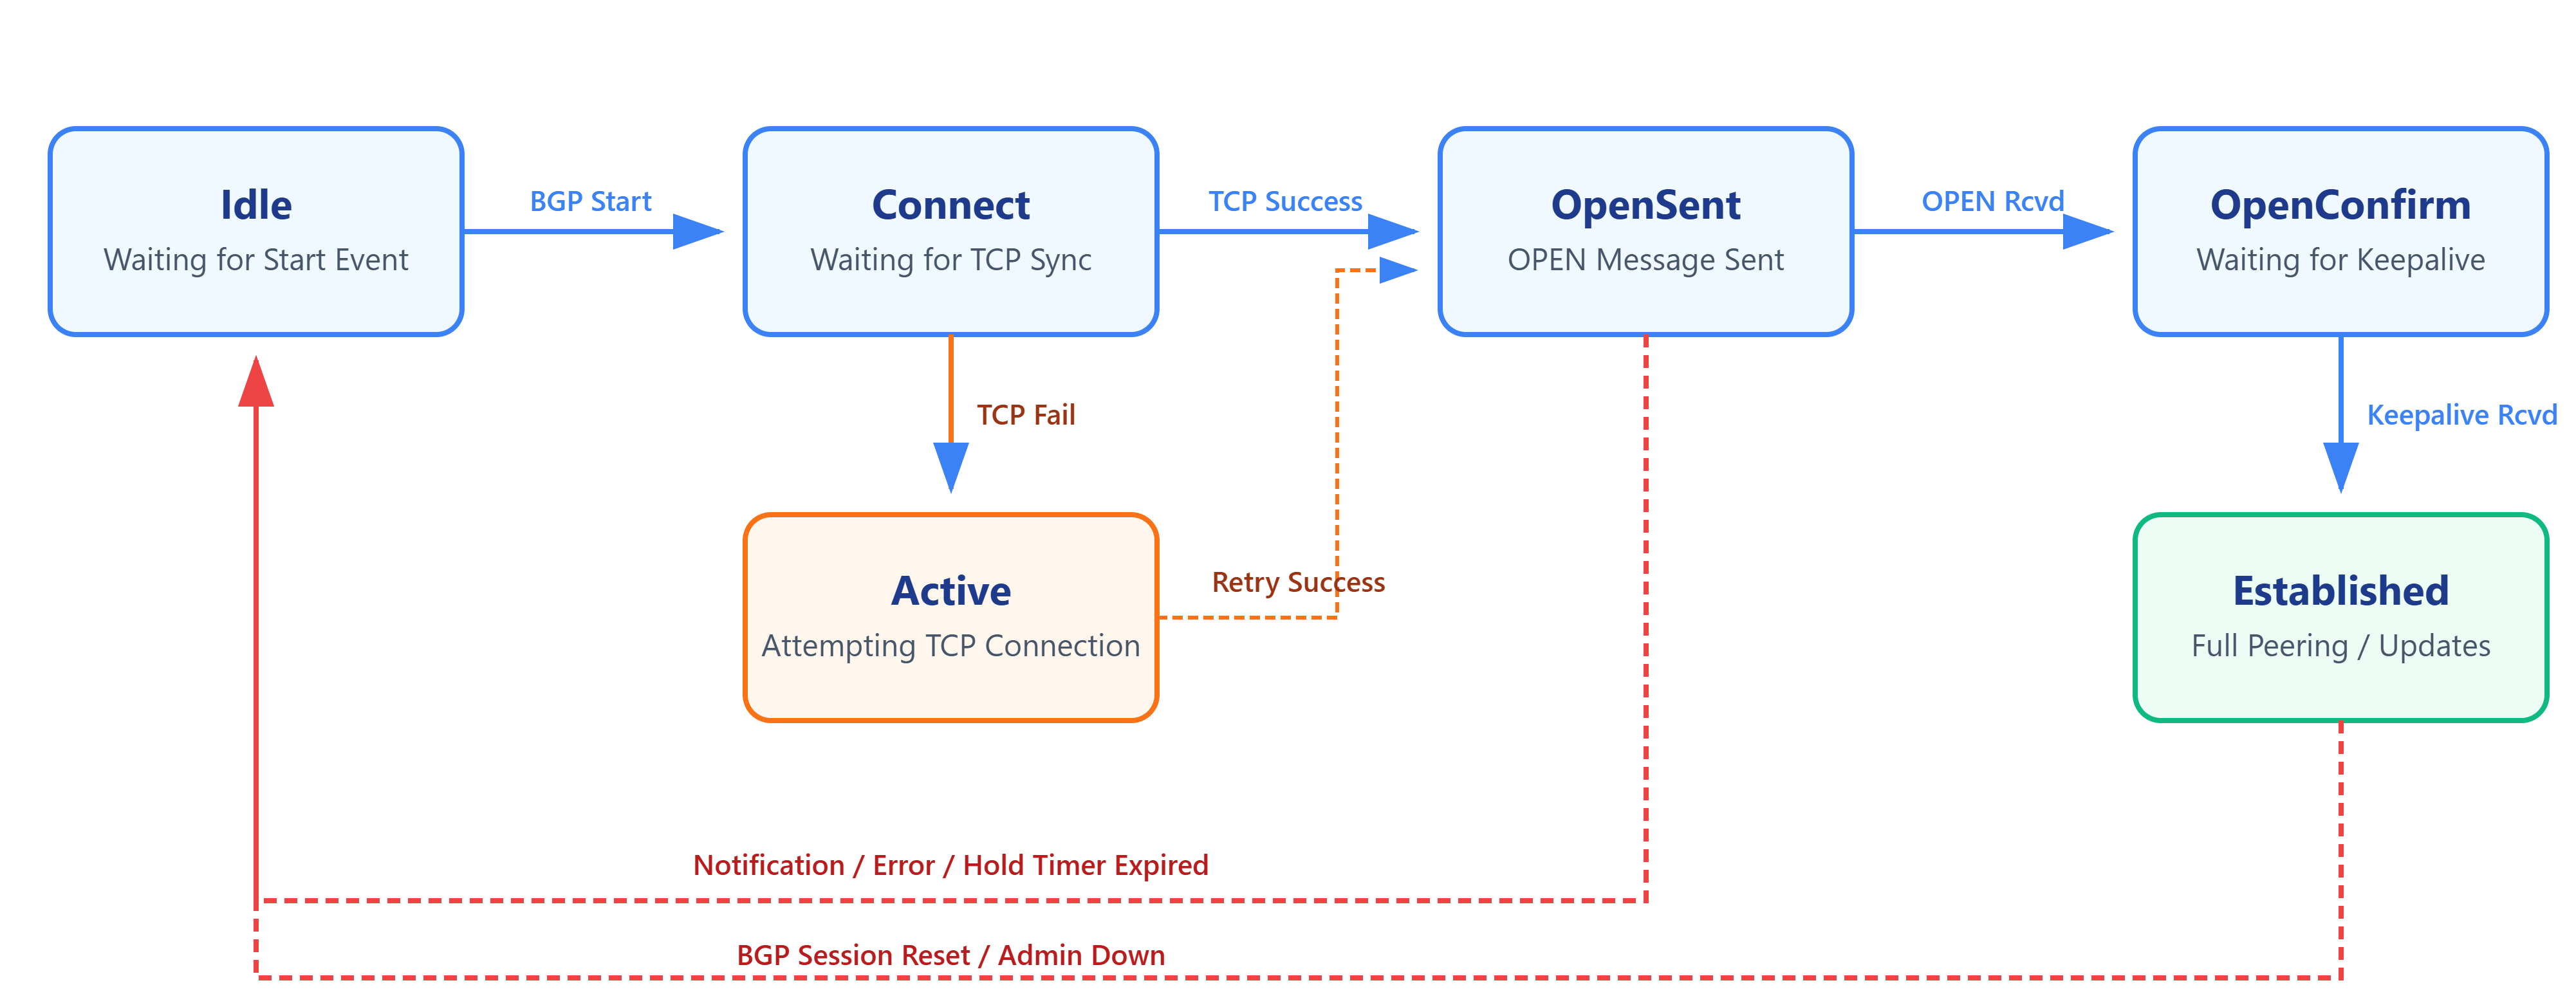
\includegraphics[width=1.0\textwidth,height=6.5cm]{Images/BGP-MFS.png}}
\newcommand{\VTEPtraffic}{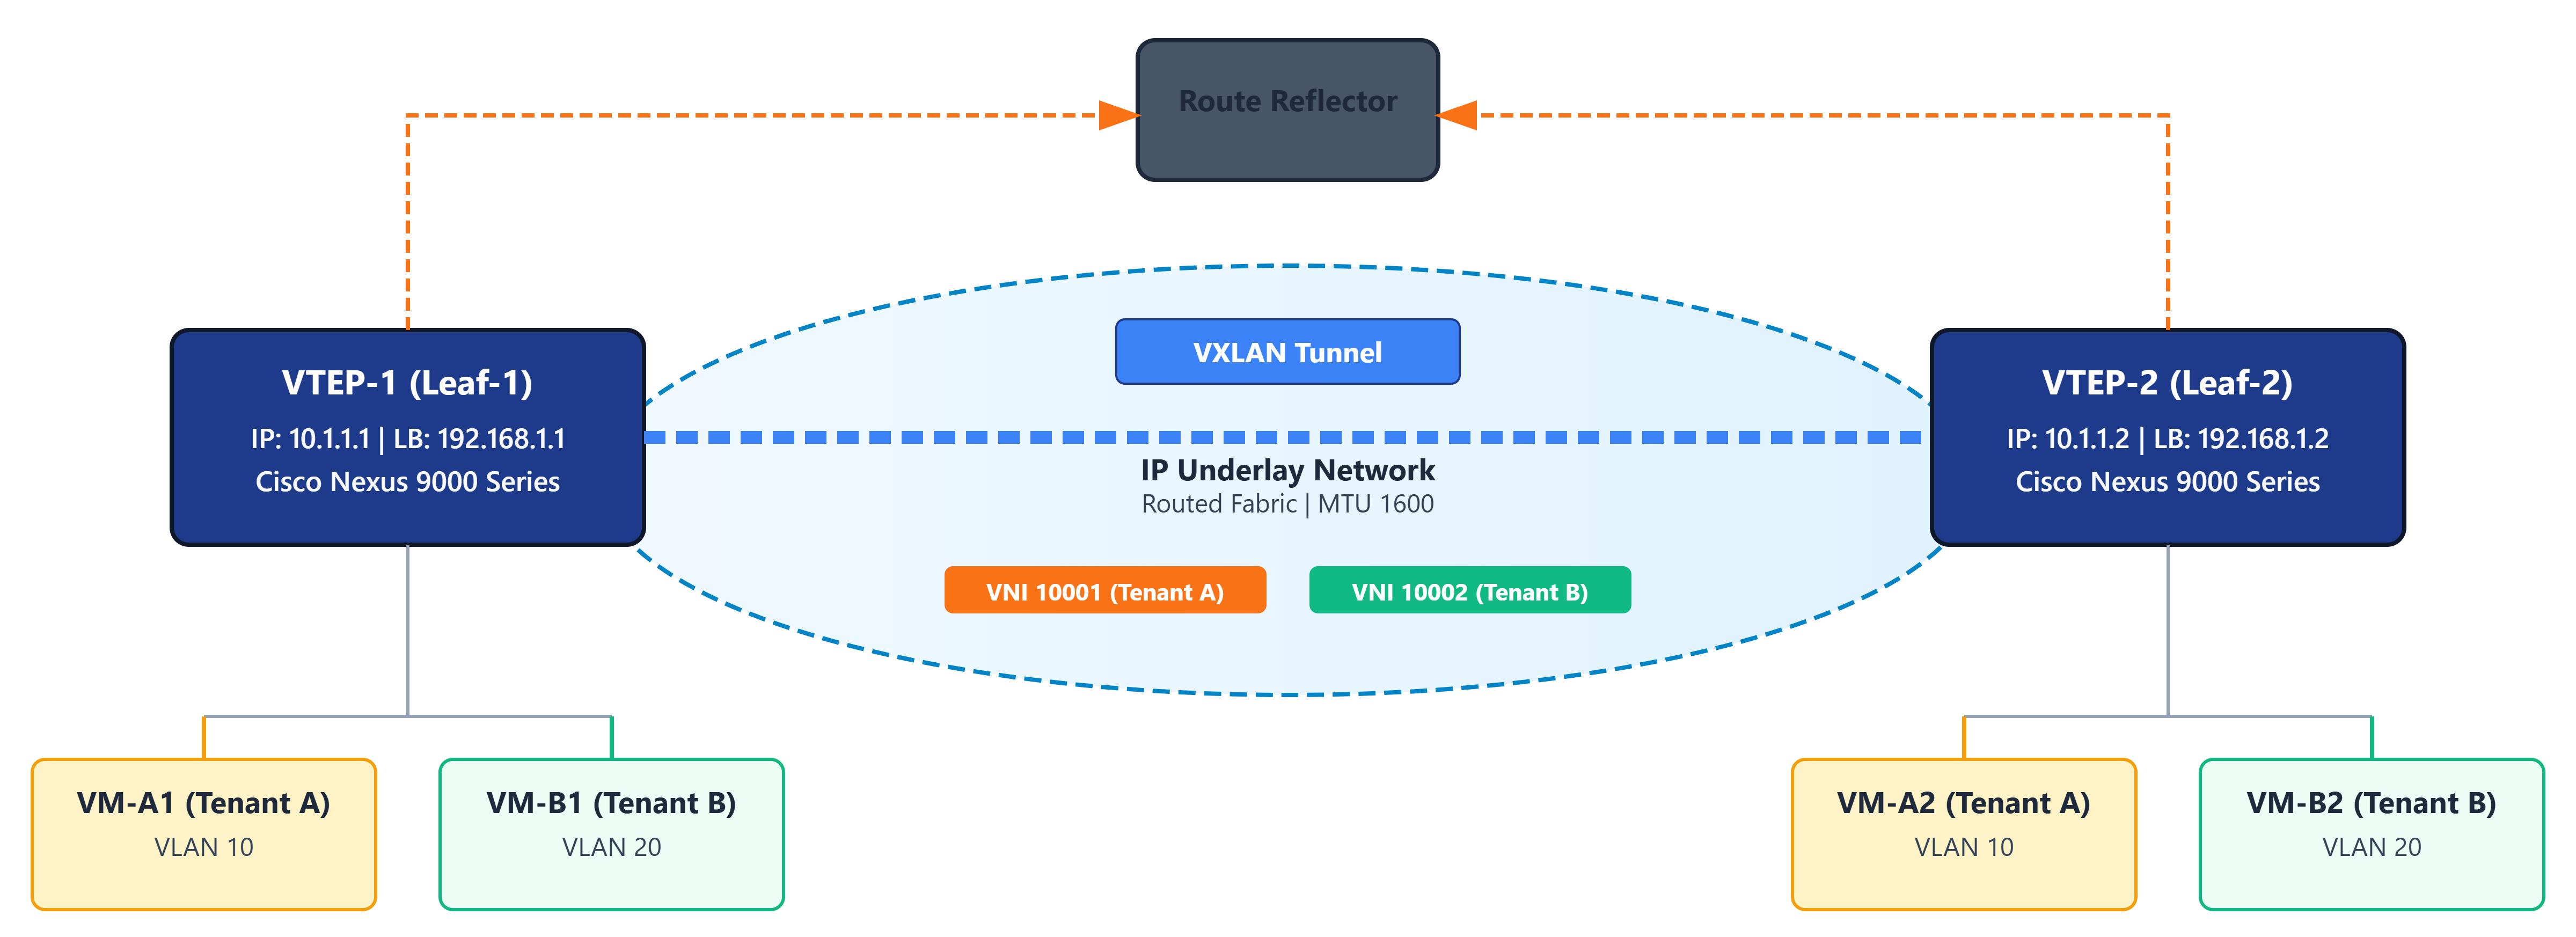
\includegraphics[width=1.0\textwidth,height=9.1cm]{Images/VTEPtraffic.png}}
\newcommand{\VXLANDiagram}{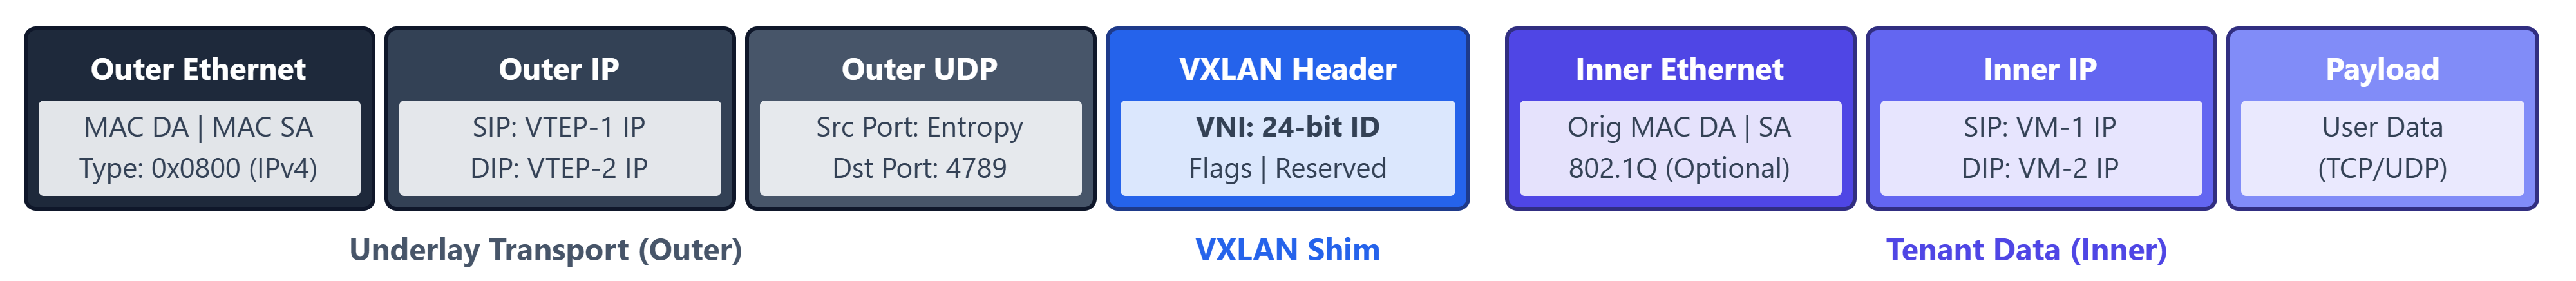
\includegraphics[width=1.0\textwidth,height=4.1cm]{Images/VXLANDiagram.png}}
\newcommand{\BumTraffic}{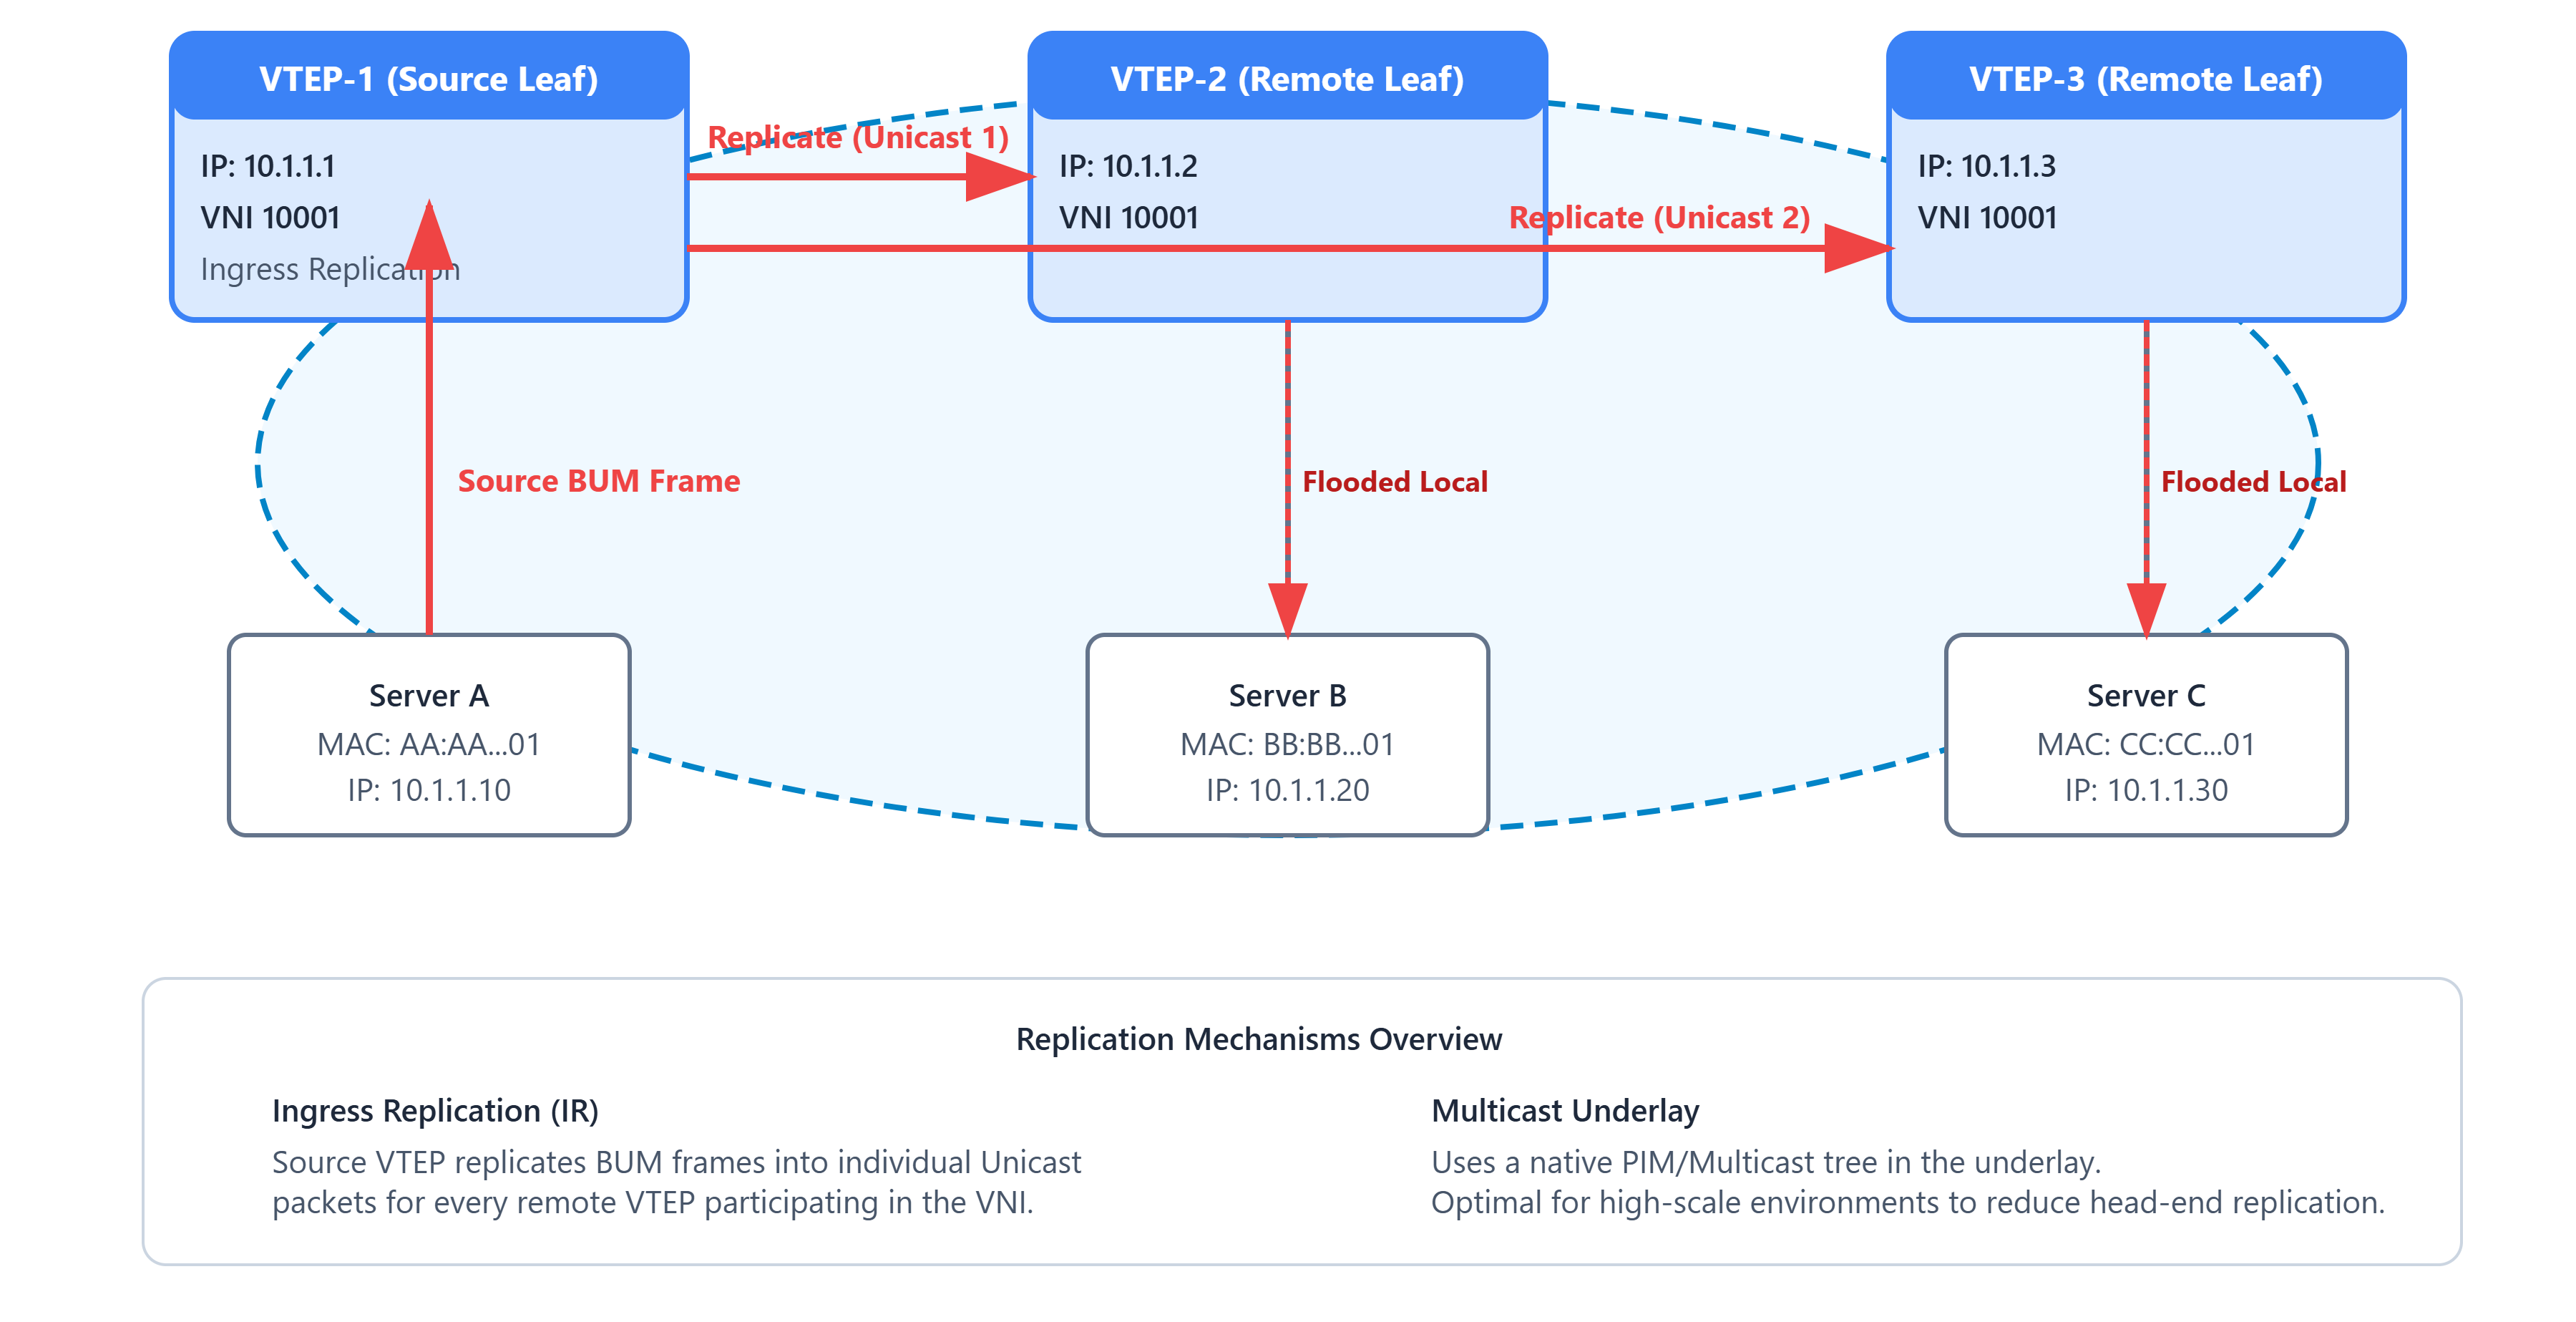
\includegraphics[width=1.0\textwidth,height=10cm]{Images/BumTraffic.png}}
\newcommand{\typeone}{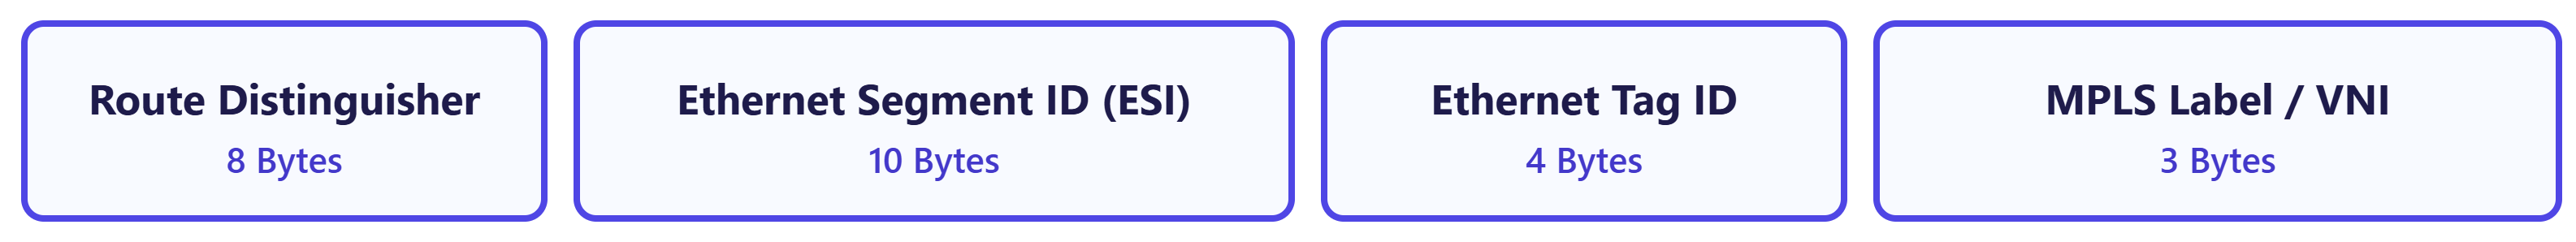
\includegraphics[width=\textwidth,height=2cm]{Images/Type1Evpn.png}}
\newcommand{\typetwo}{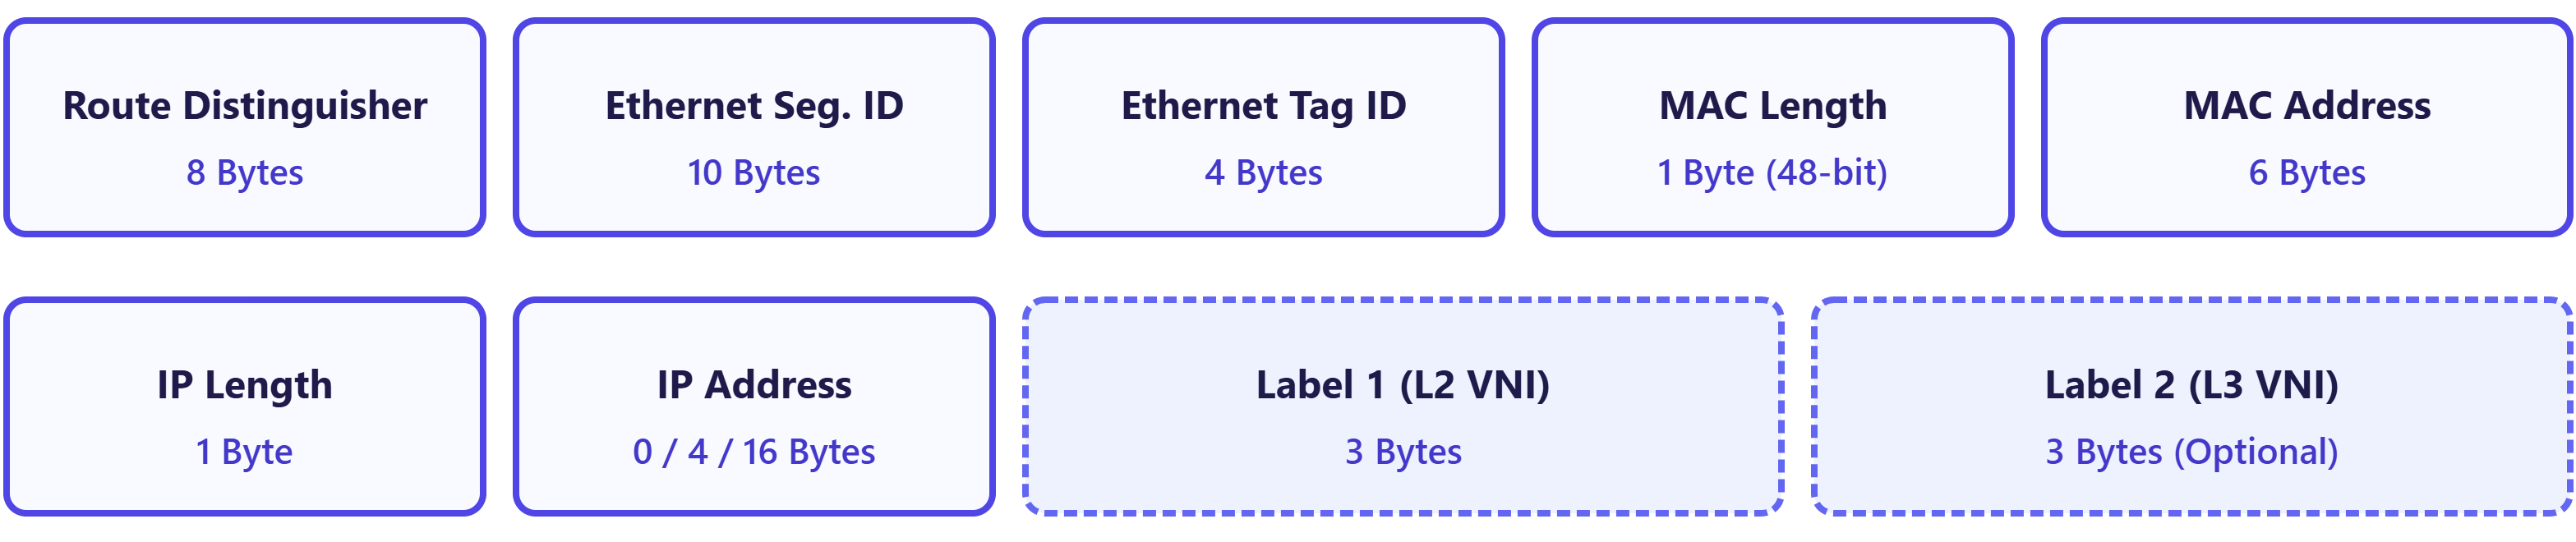
\includegraphics[width=\textwidth,height=3.5cm]{Images/Type2Evpn.png}}
\newcommand{\typethree}{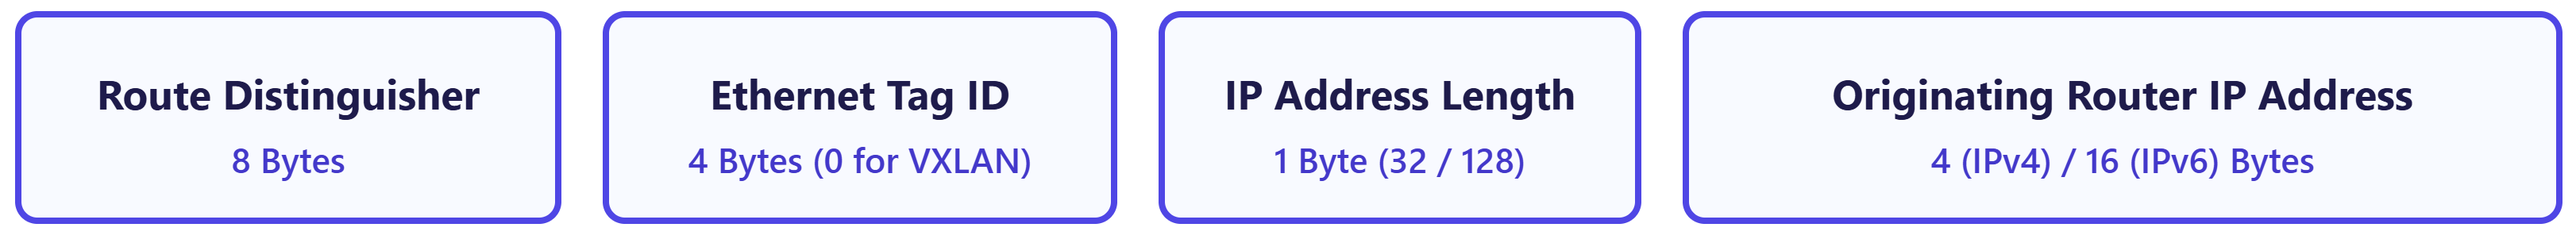
\includegraphics[width=\textwidth,height=2cm]{Images/Type3Evpn.png}}
\newcommand{\typefour}{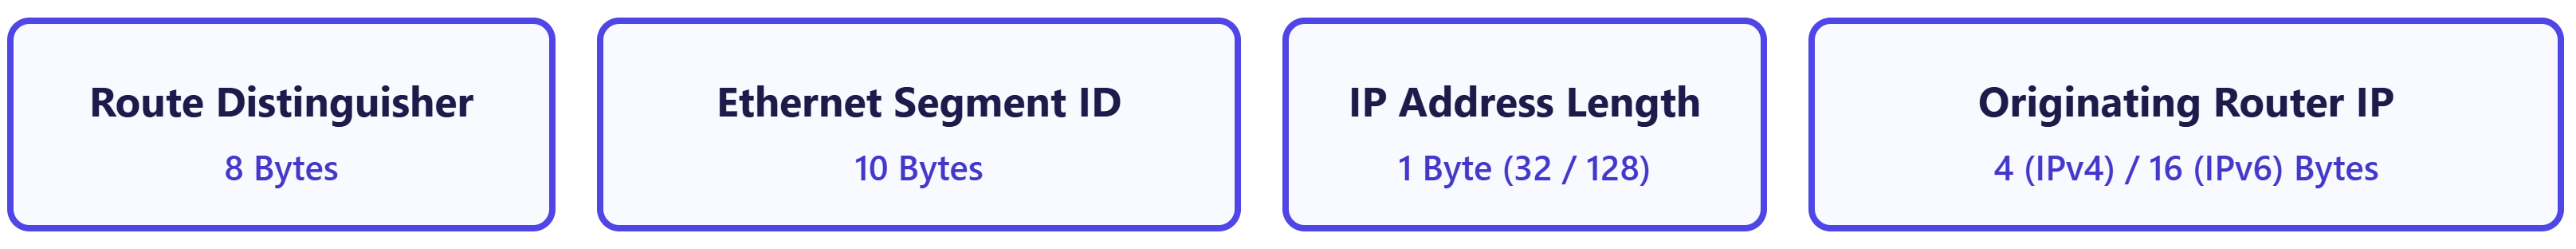
\includegraphics[width=\textwidth,height=2cm]{Images/Type4Evpn.png}}
\newcommand{\typefive}{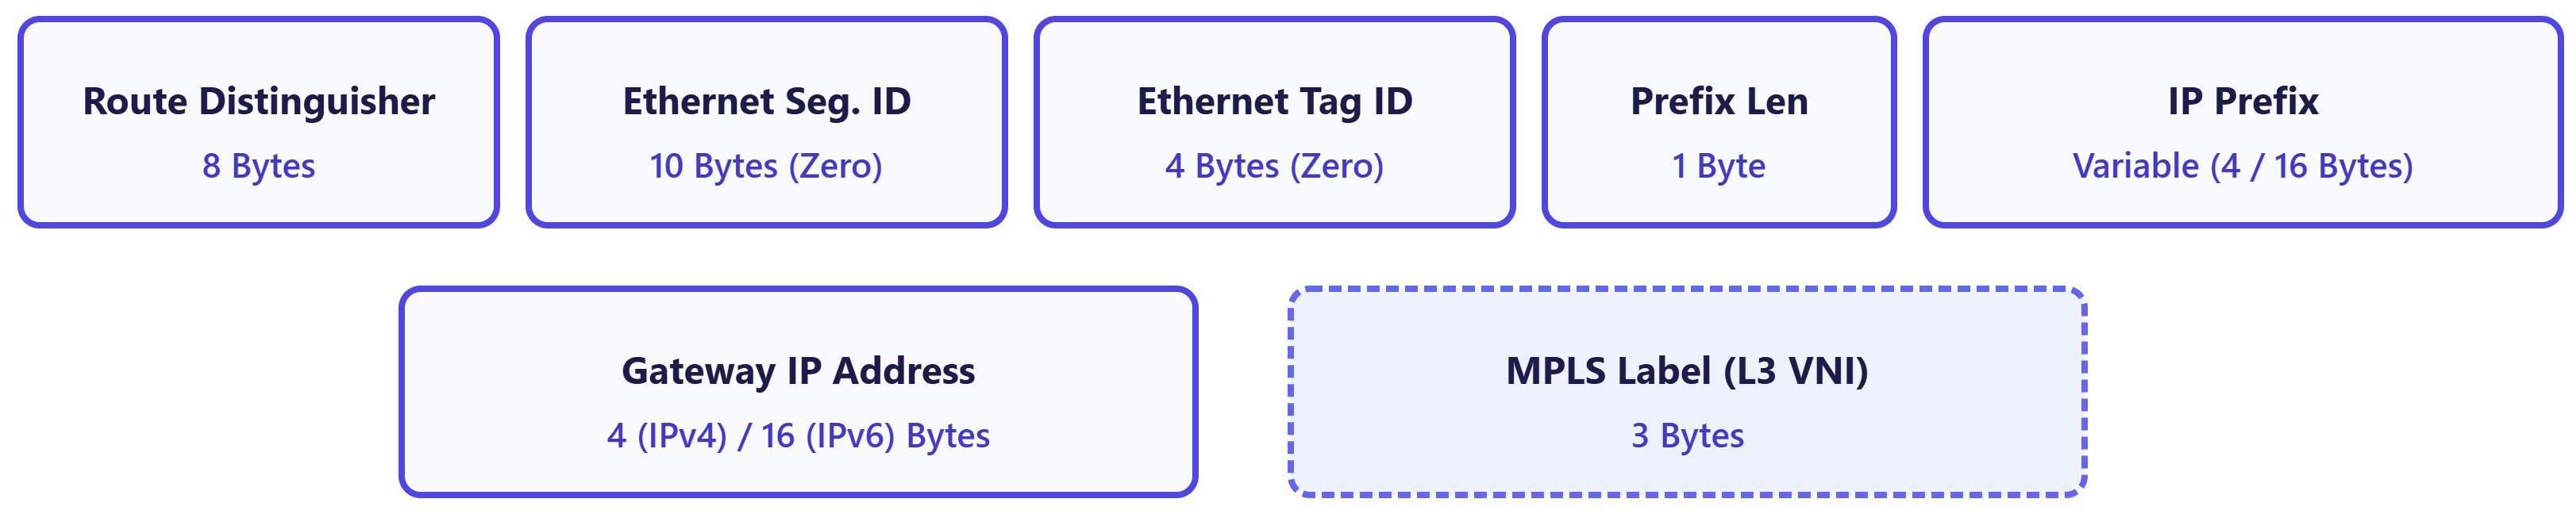
\includegraphics[width=\textwidth,height=3.3cm]{Images/Type5Evpn.png}}
\newcommand{\EvpnDrivesVXLan}{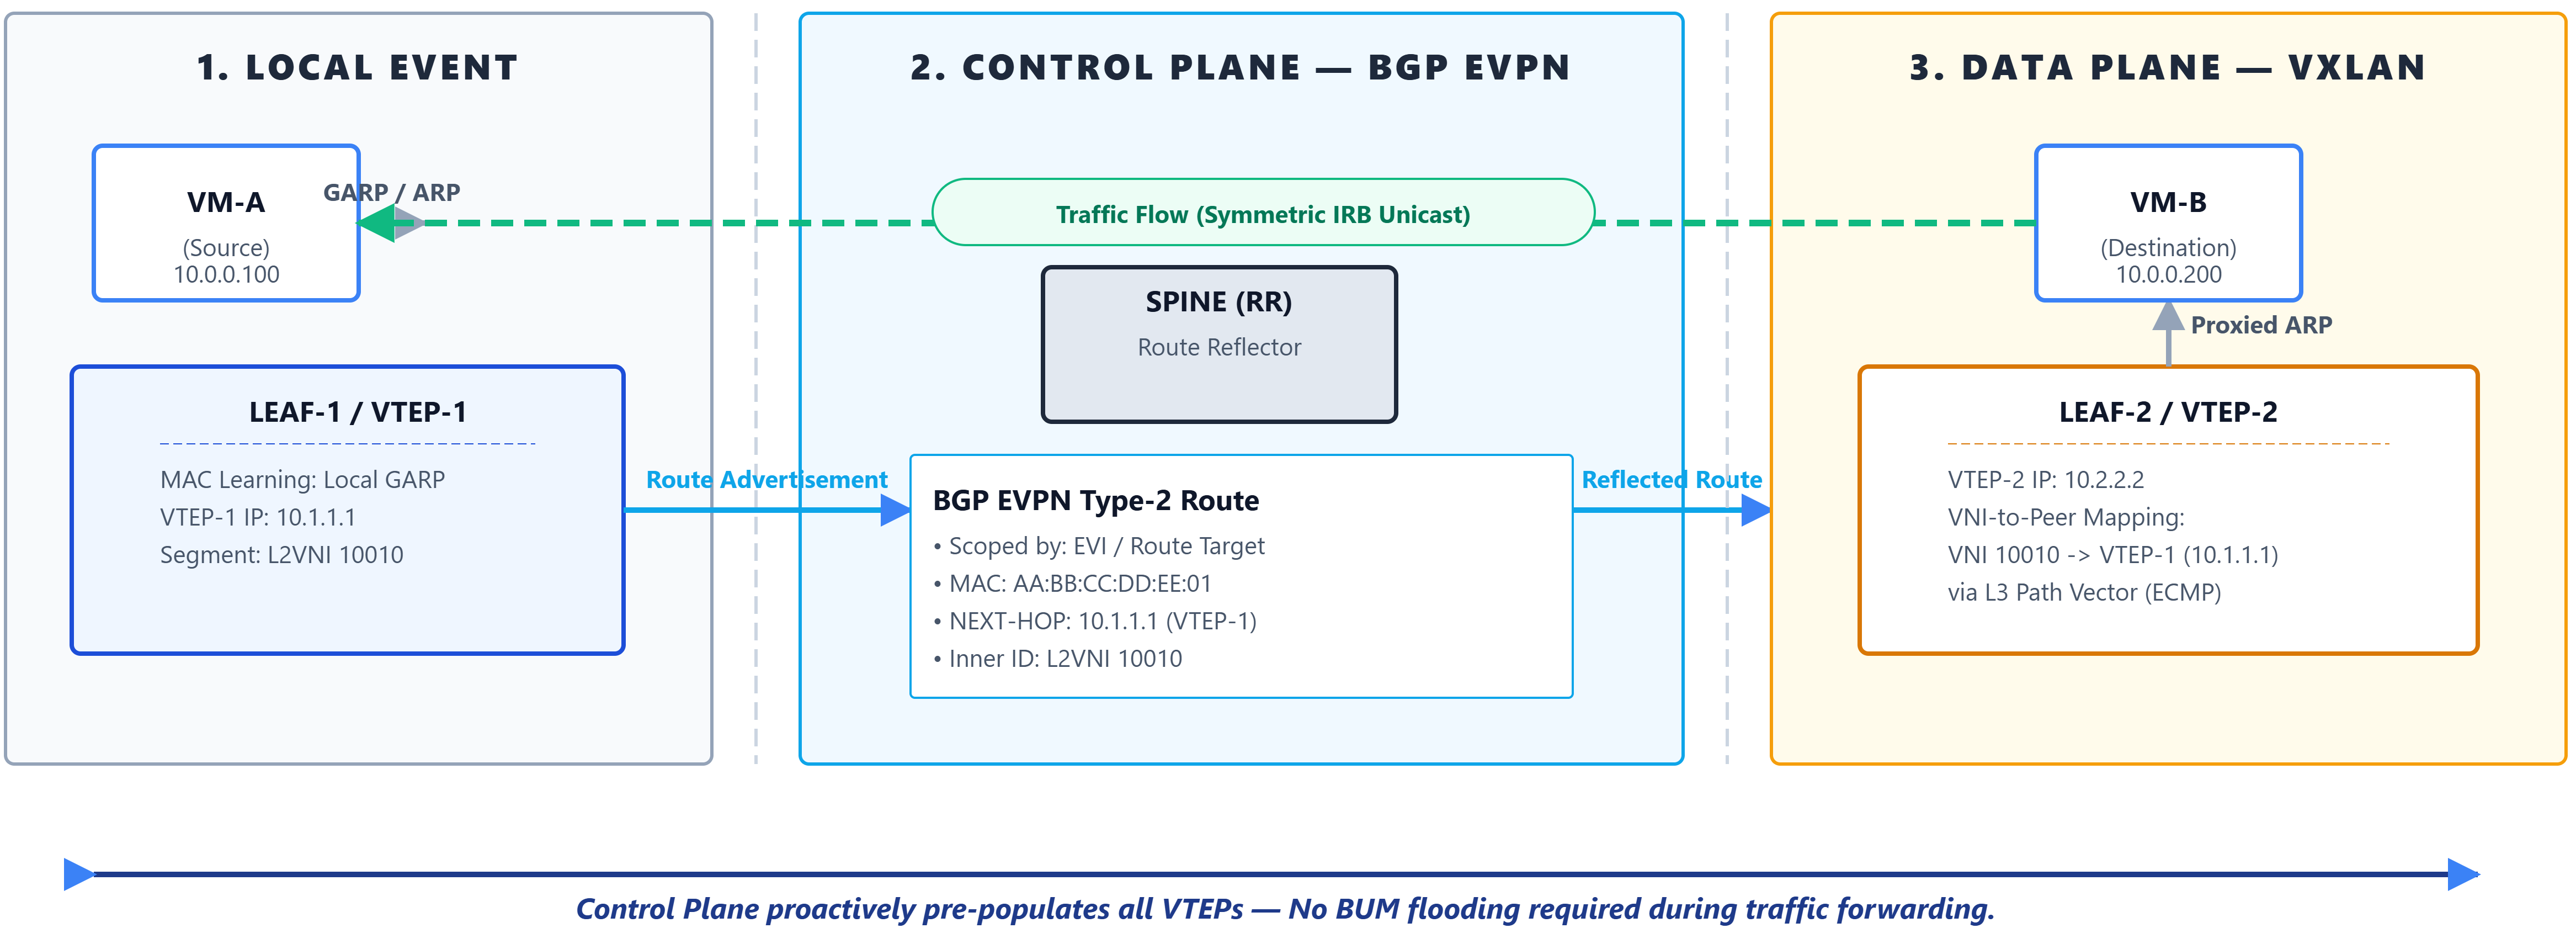
\includegraphics[width=1.0\textwidth,height=5cm]{Images/EvpnDrivesVXLan.png}}
\newcommand{\ebgpibgp}{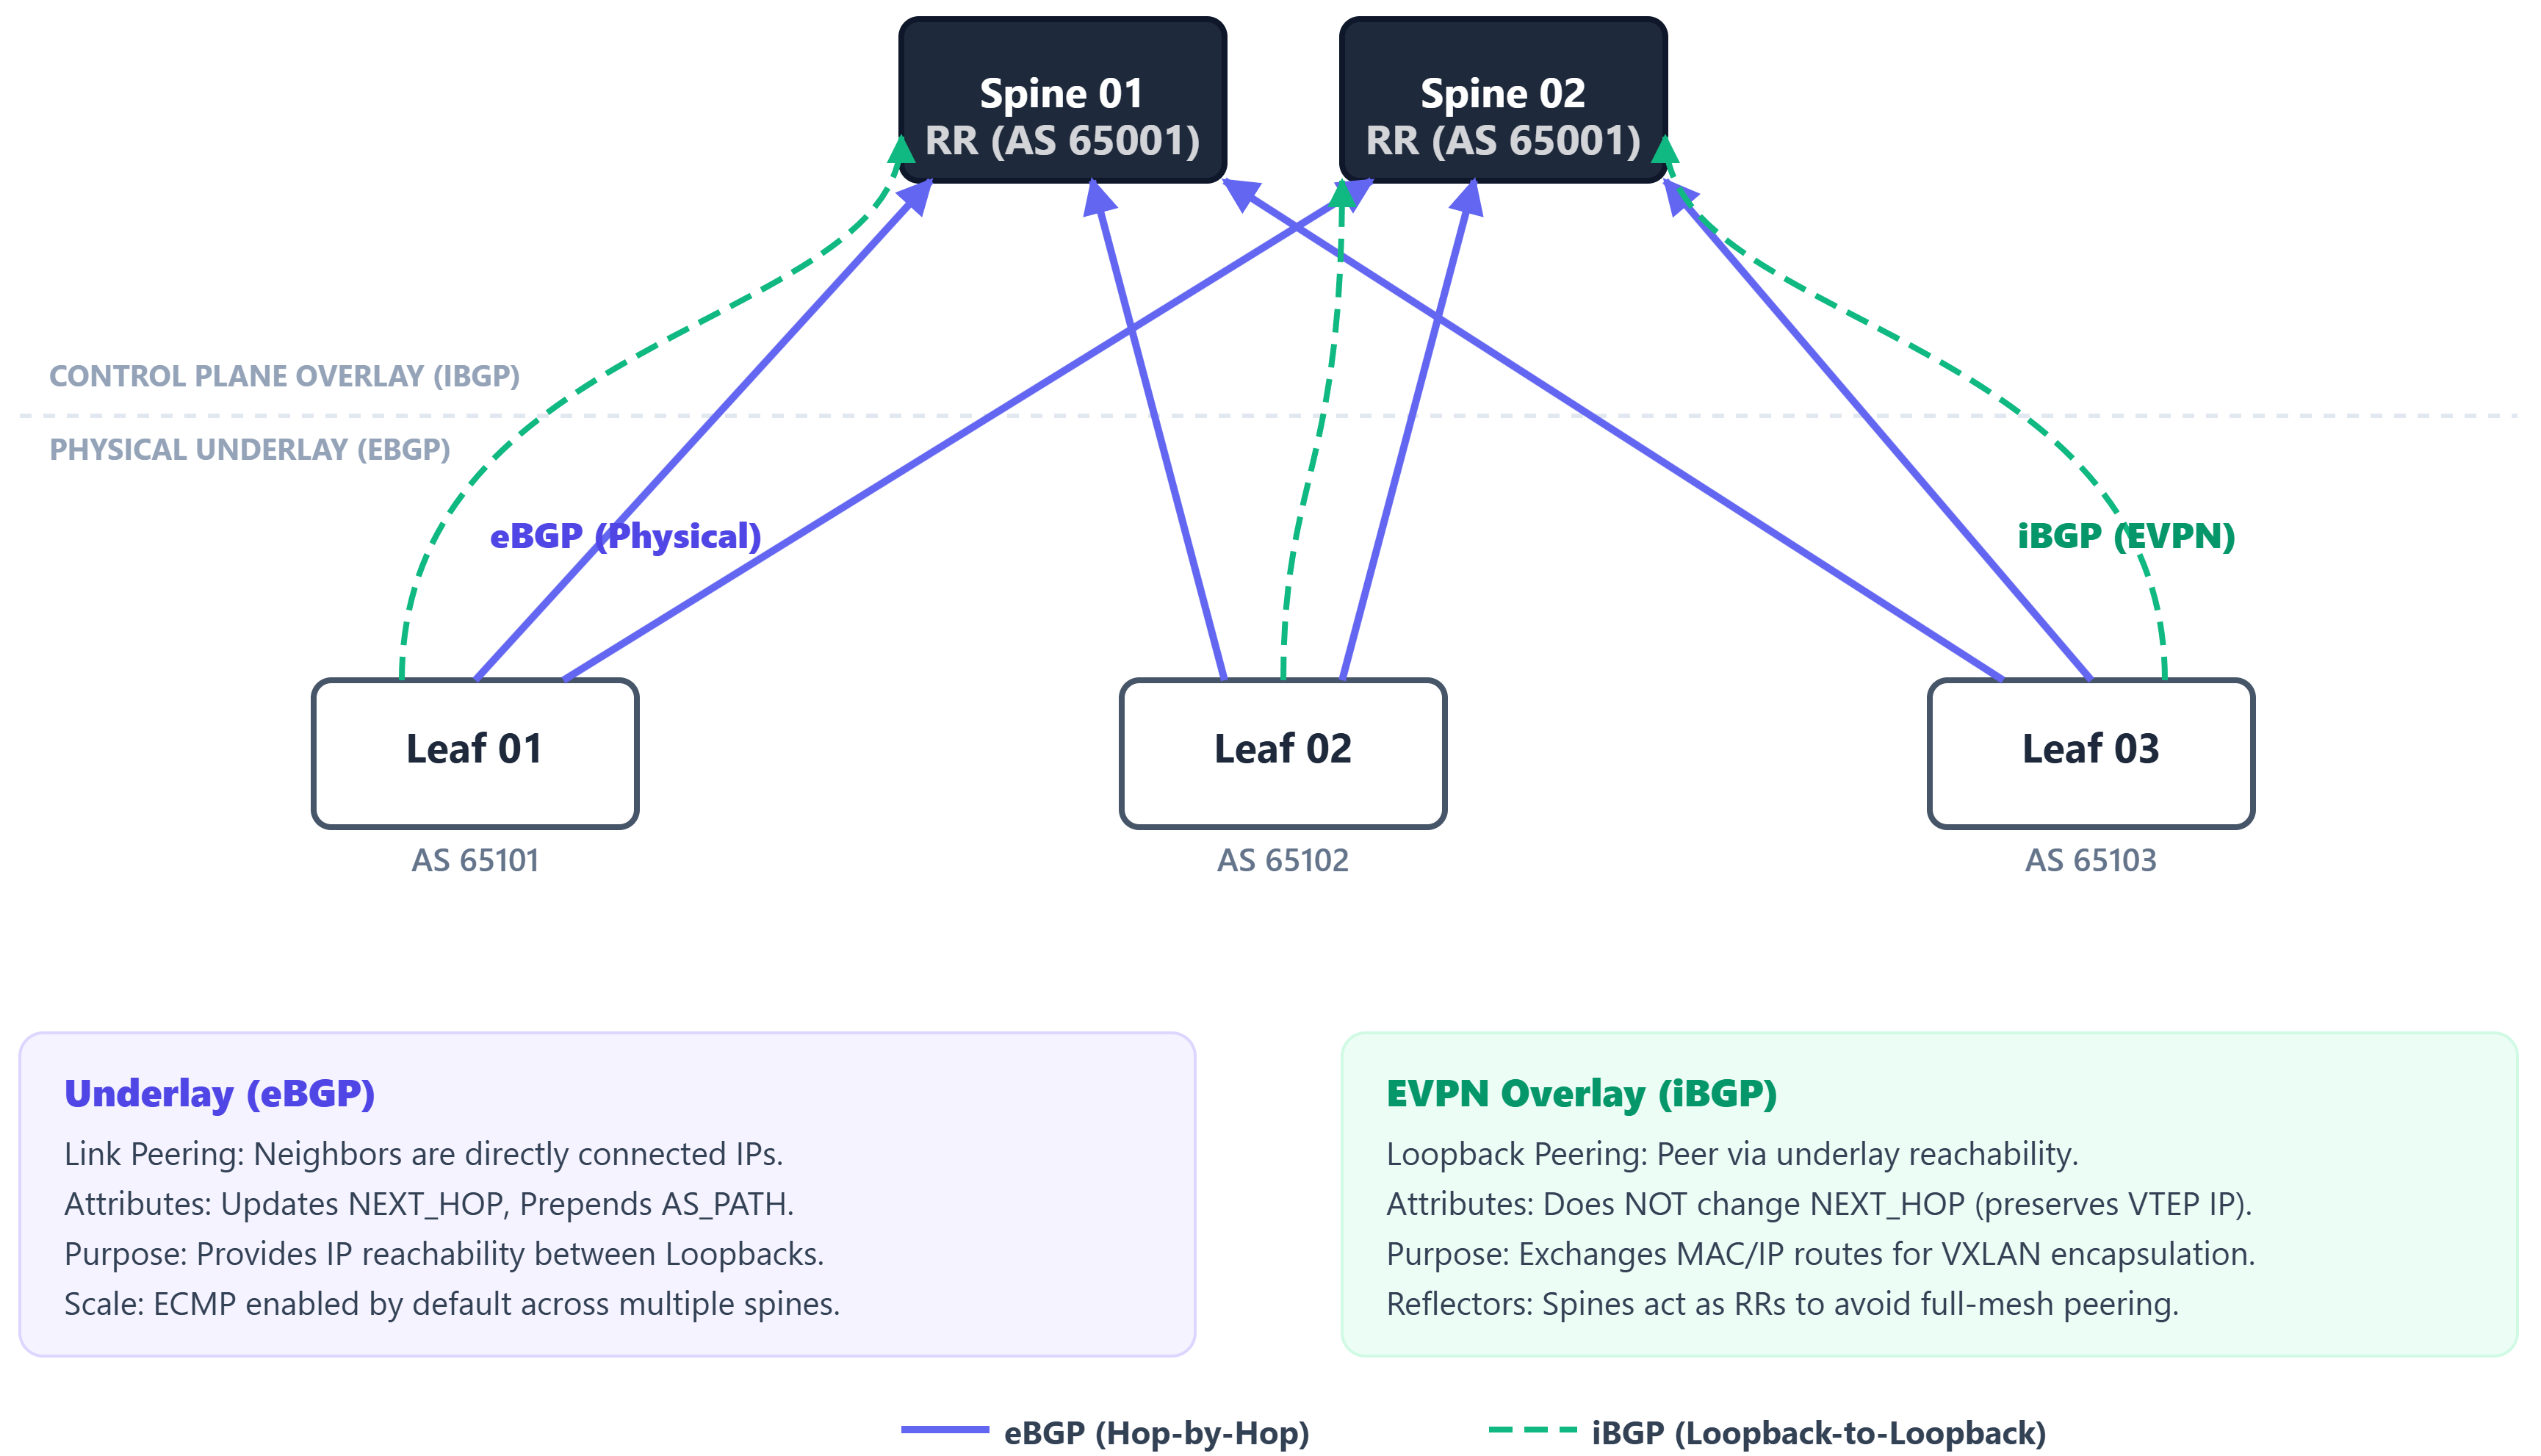
\includegraphics[width=\textwidth,height=7cm]{Images/ebgp-ibgp.png}}
\newcommand{\MACmobility}{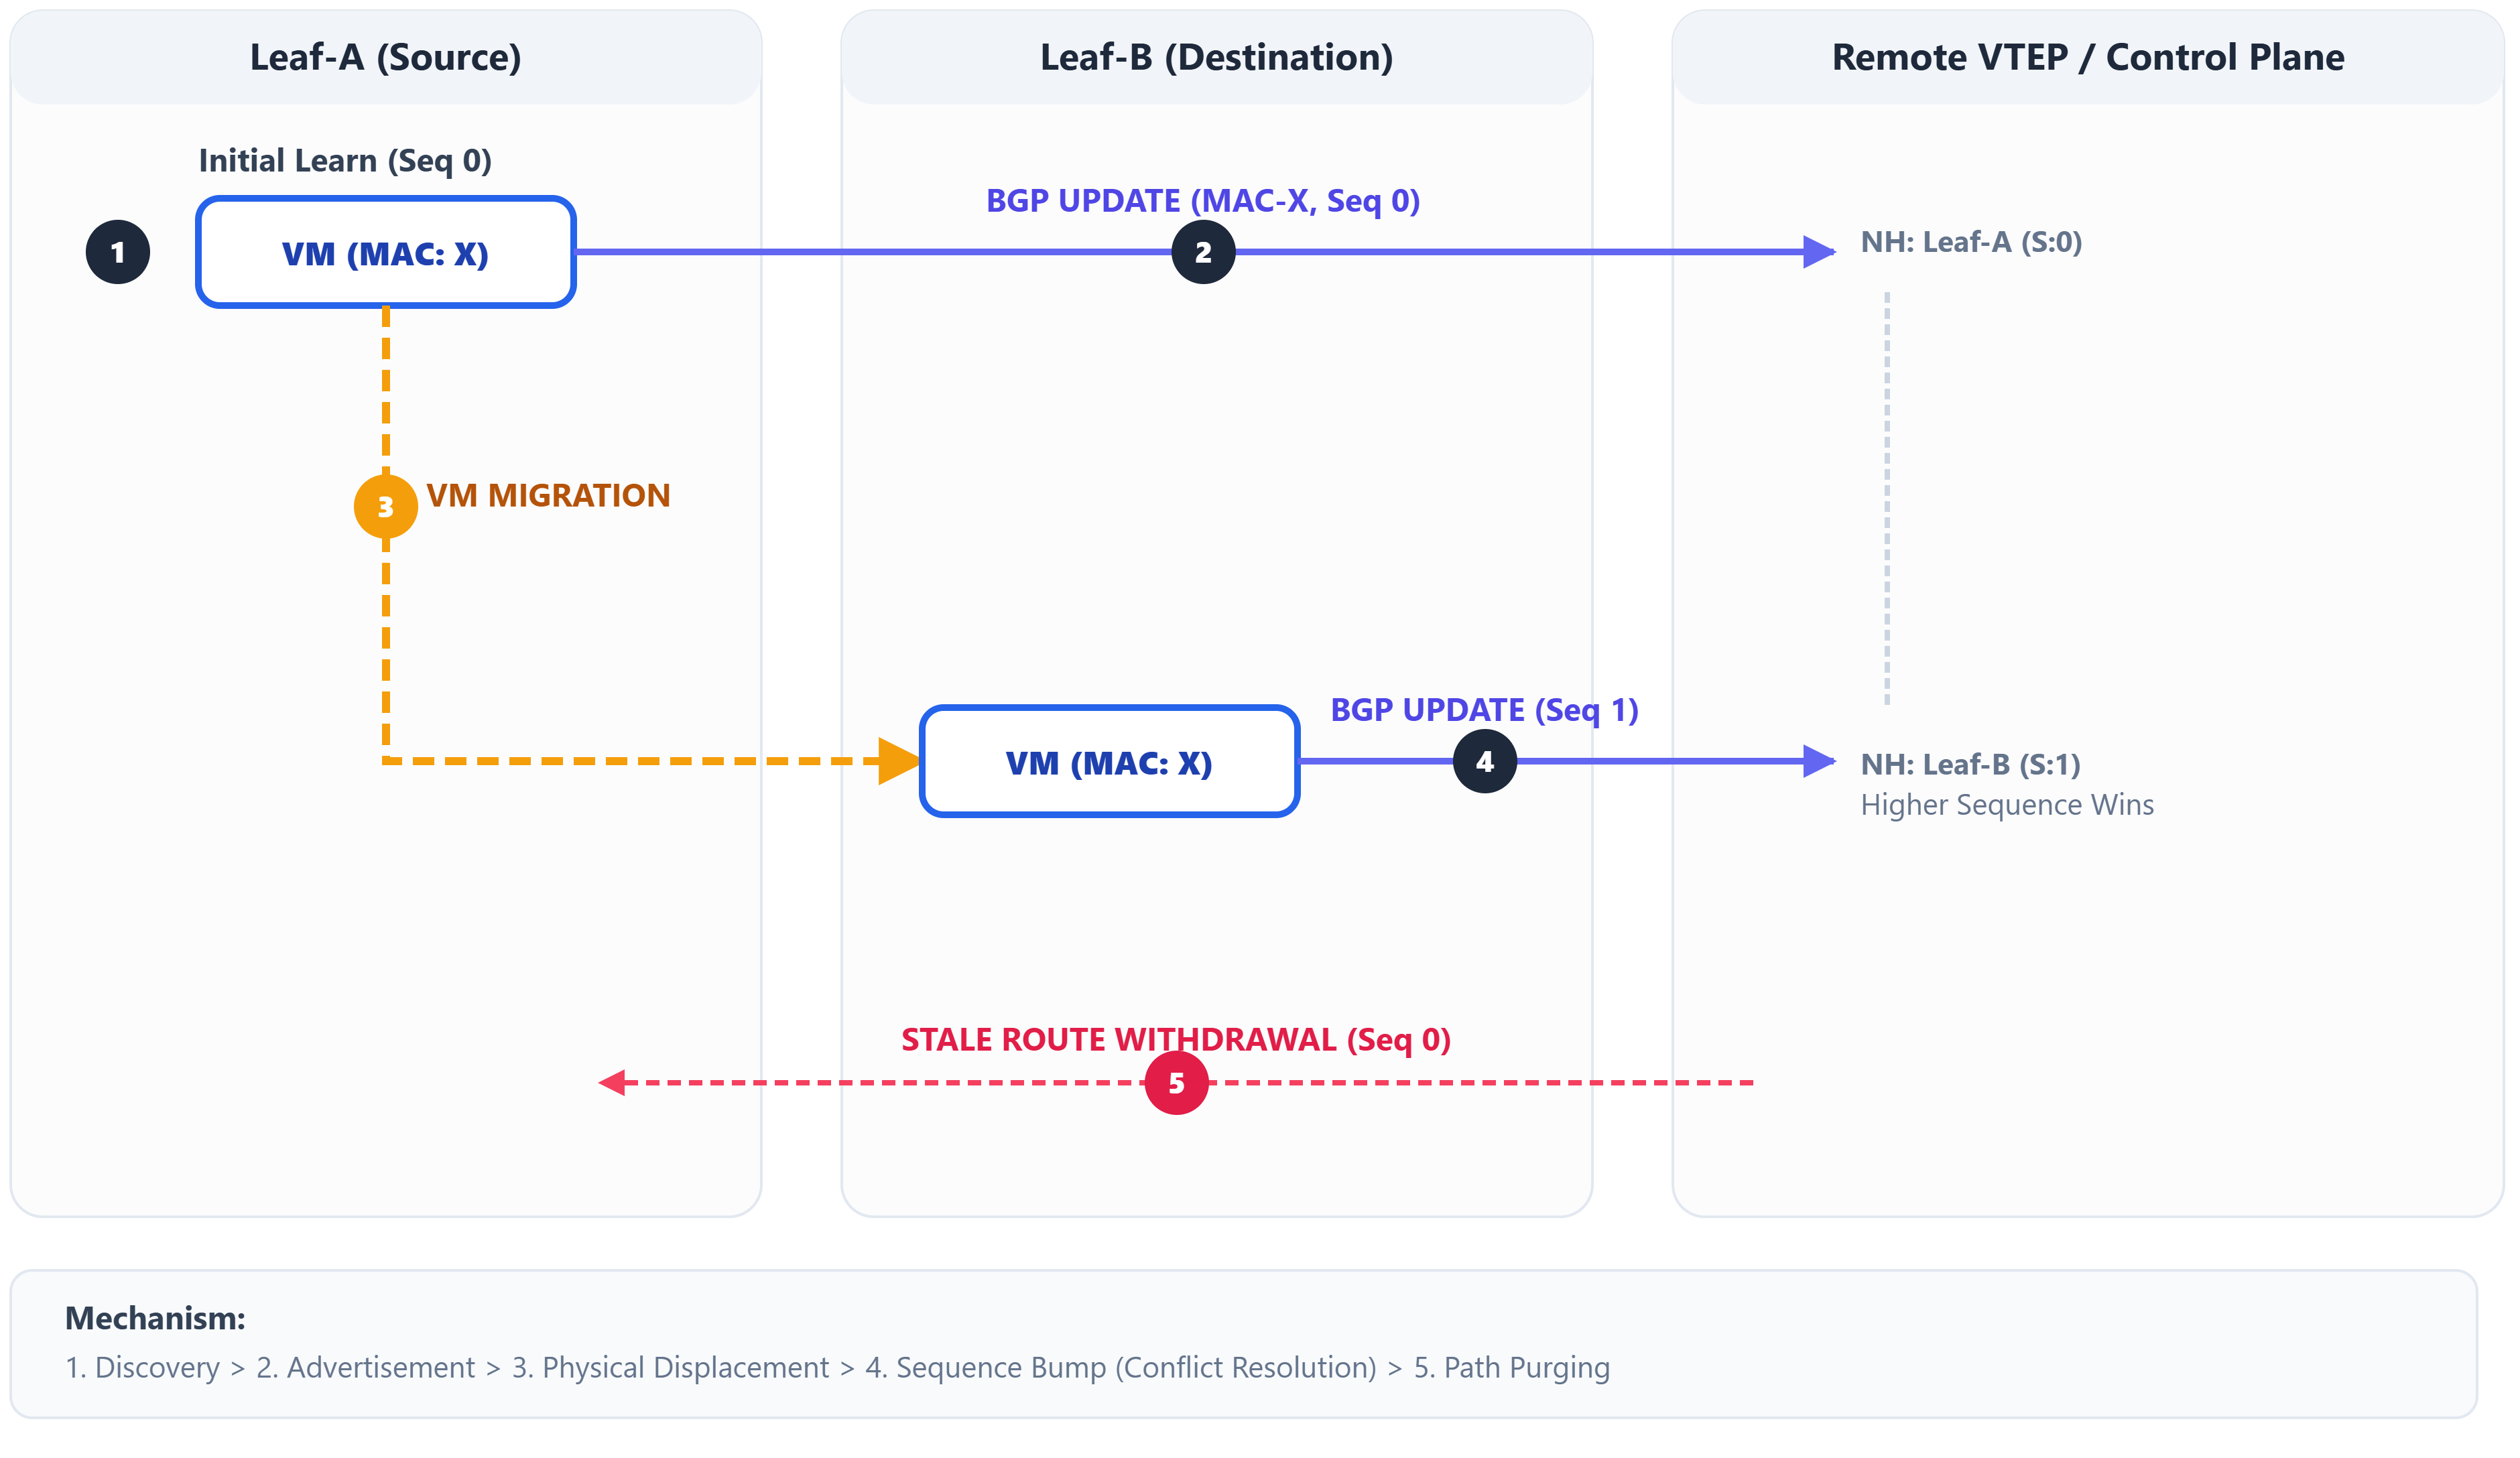
\includegraphics[width=\textwidth,height=5.5cm]{Images/MACmobility.png}}
\newcommand{\LVNILVNI}{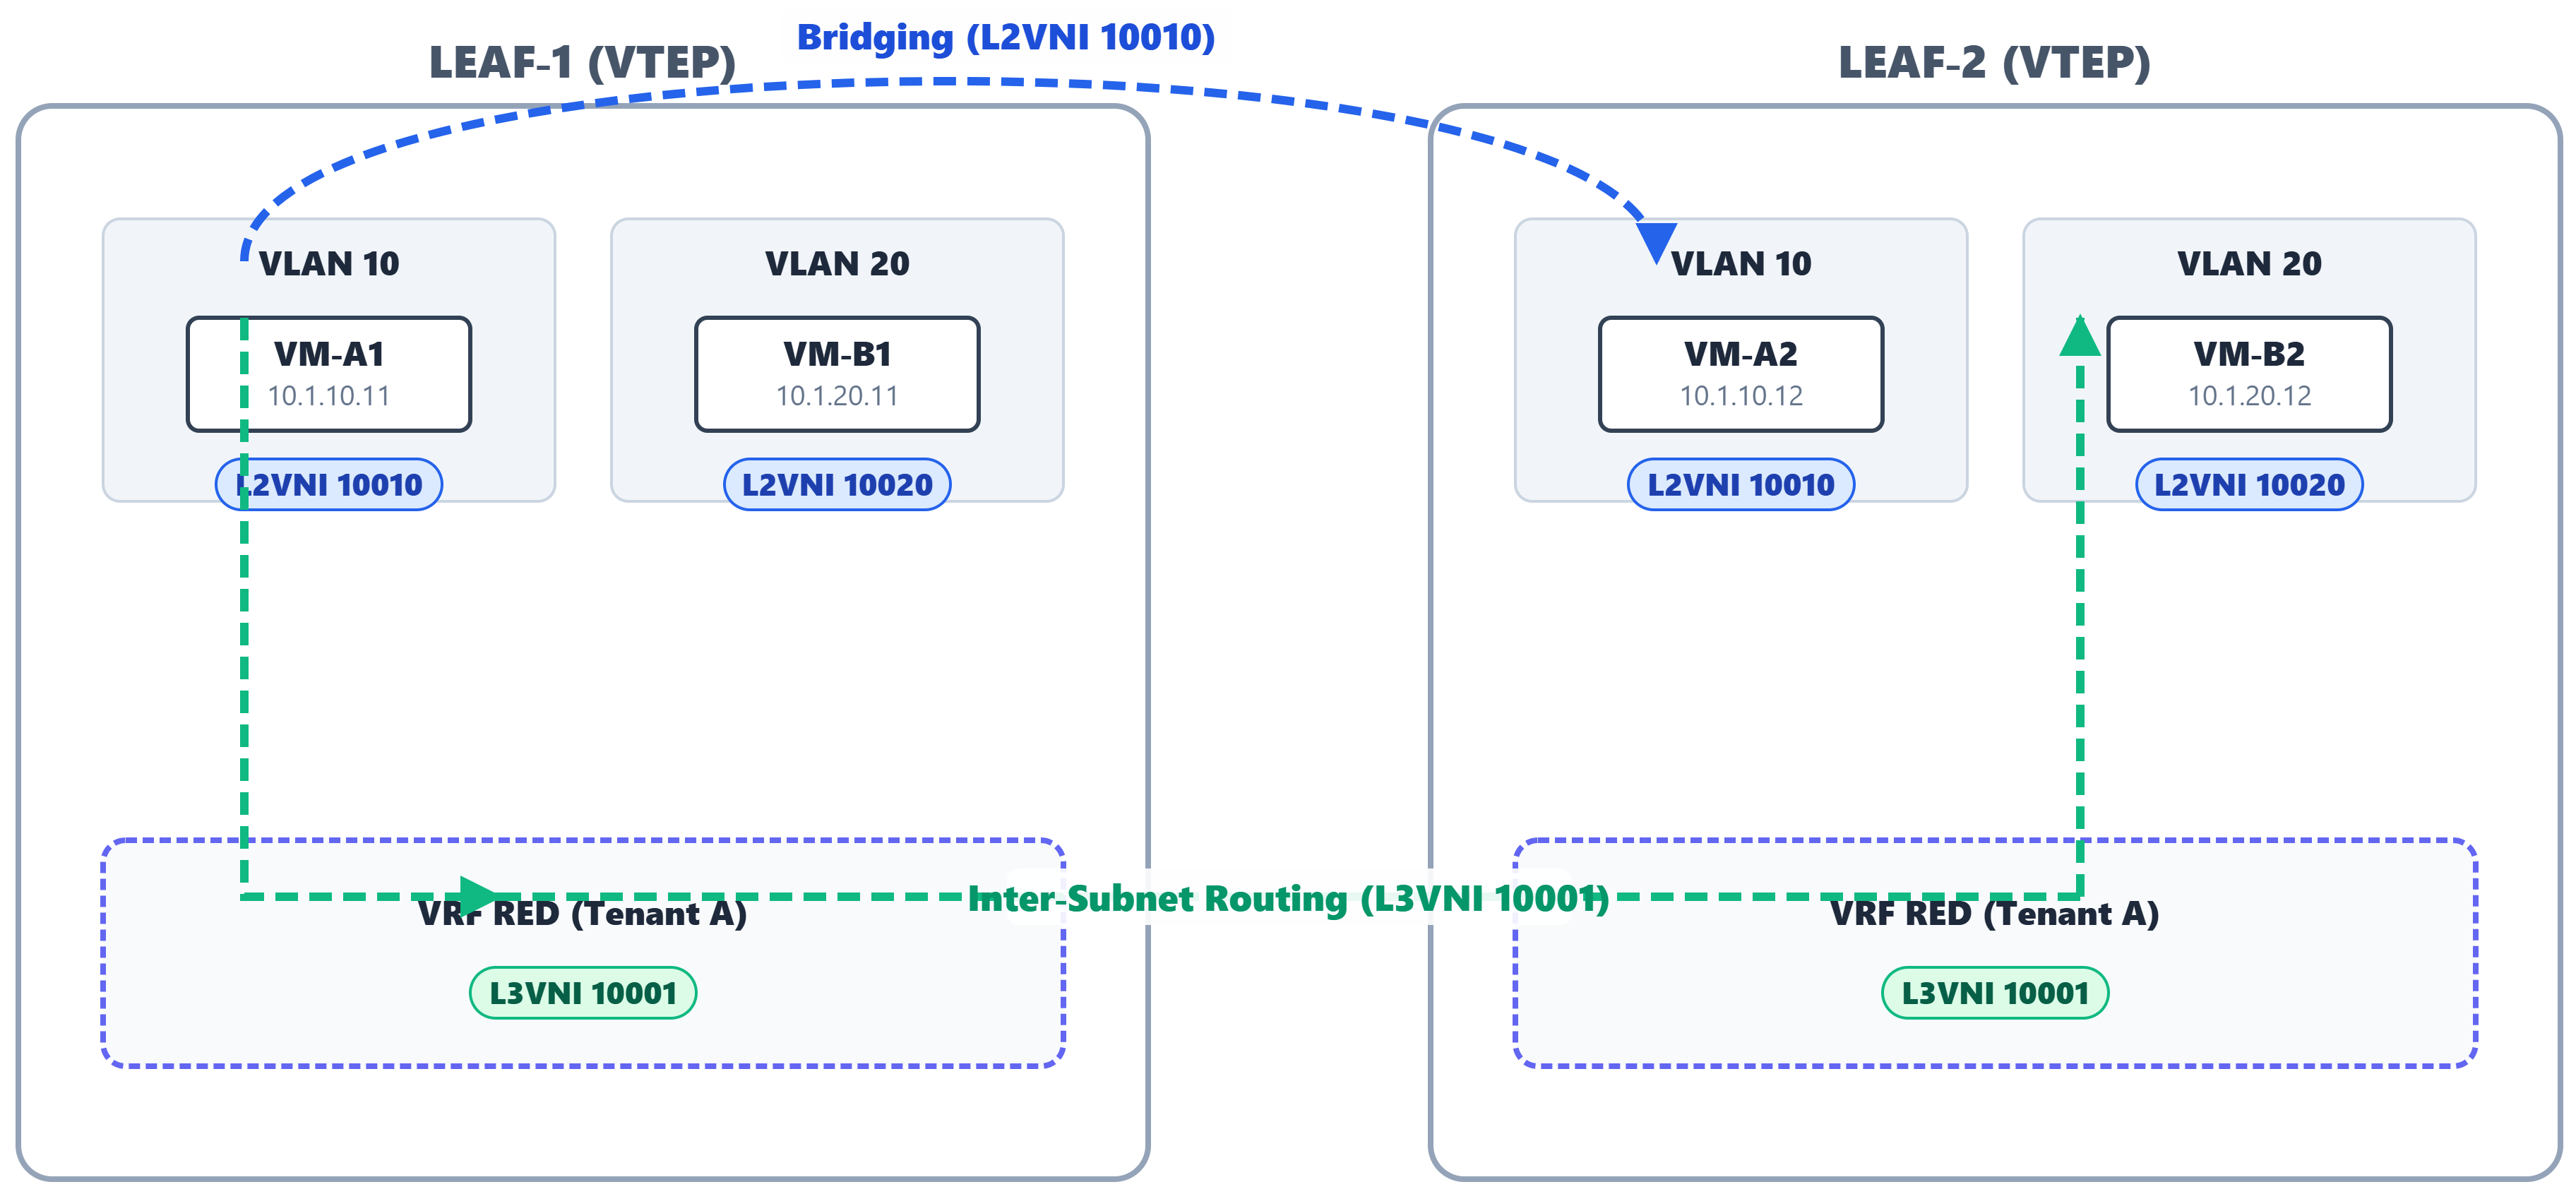
\includegraphics[width=\textwidth,height=8cm]{Images/L2VNIL3VNI.png}}
\newcommand{\AnycastGateway}{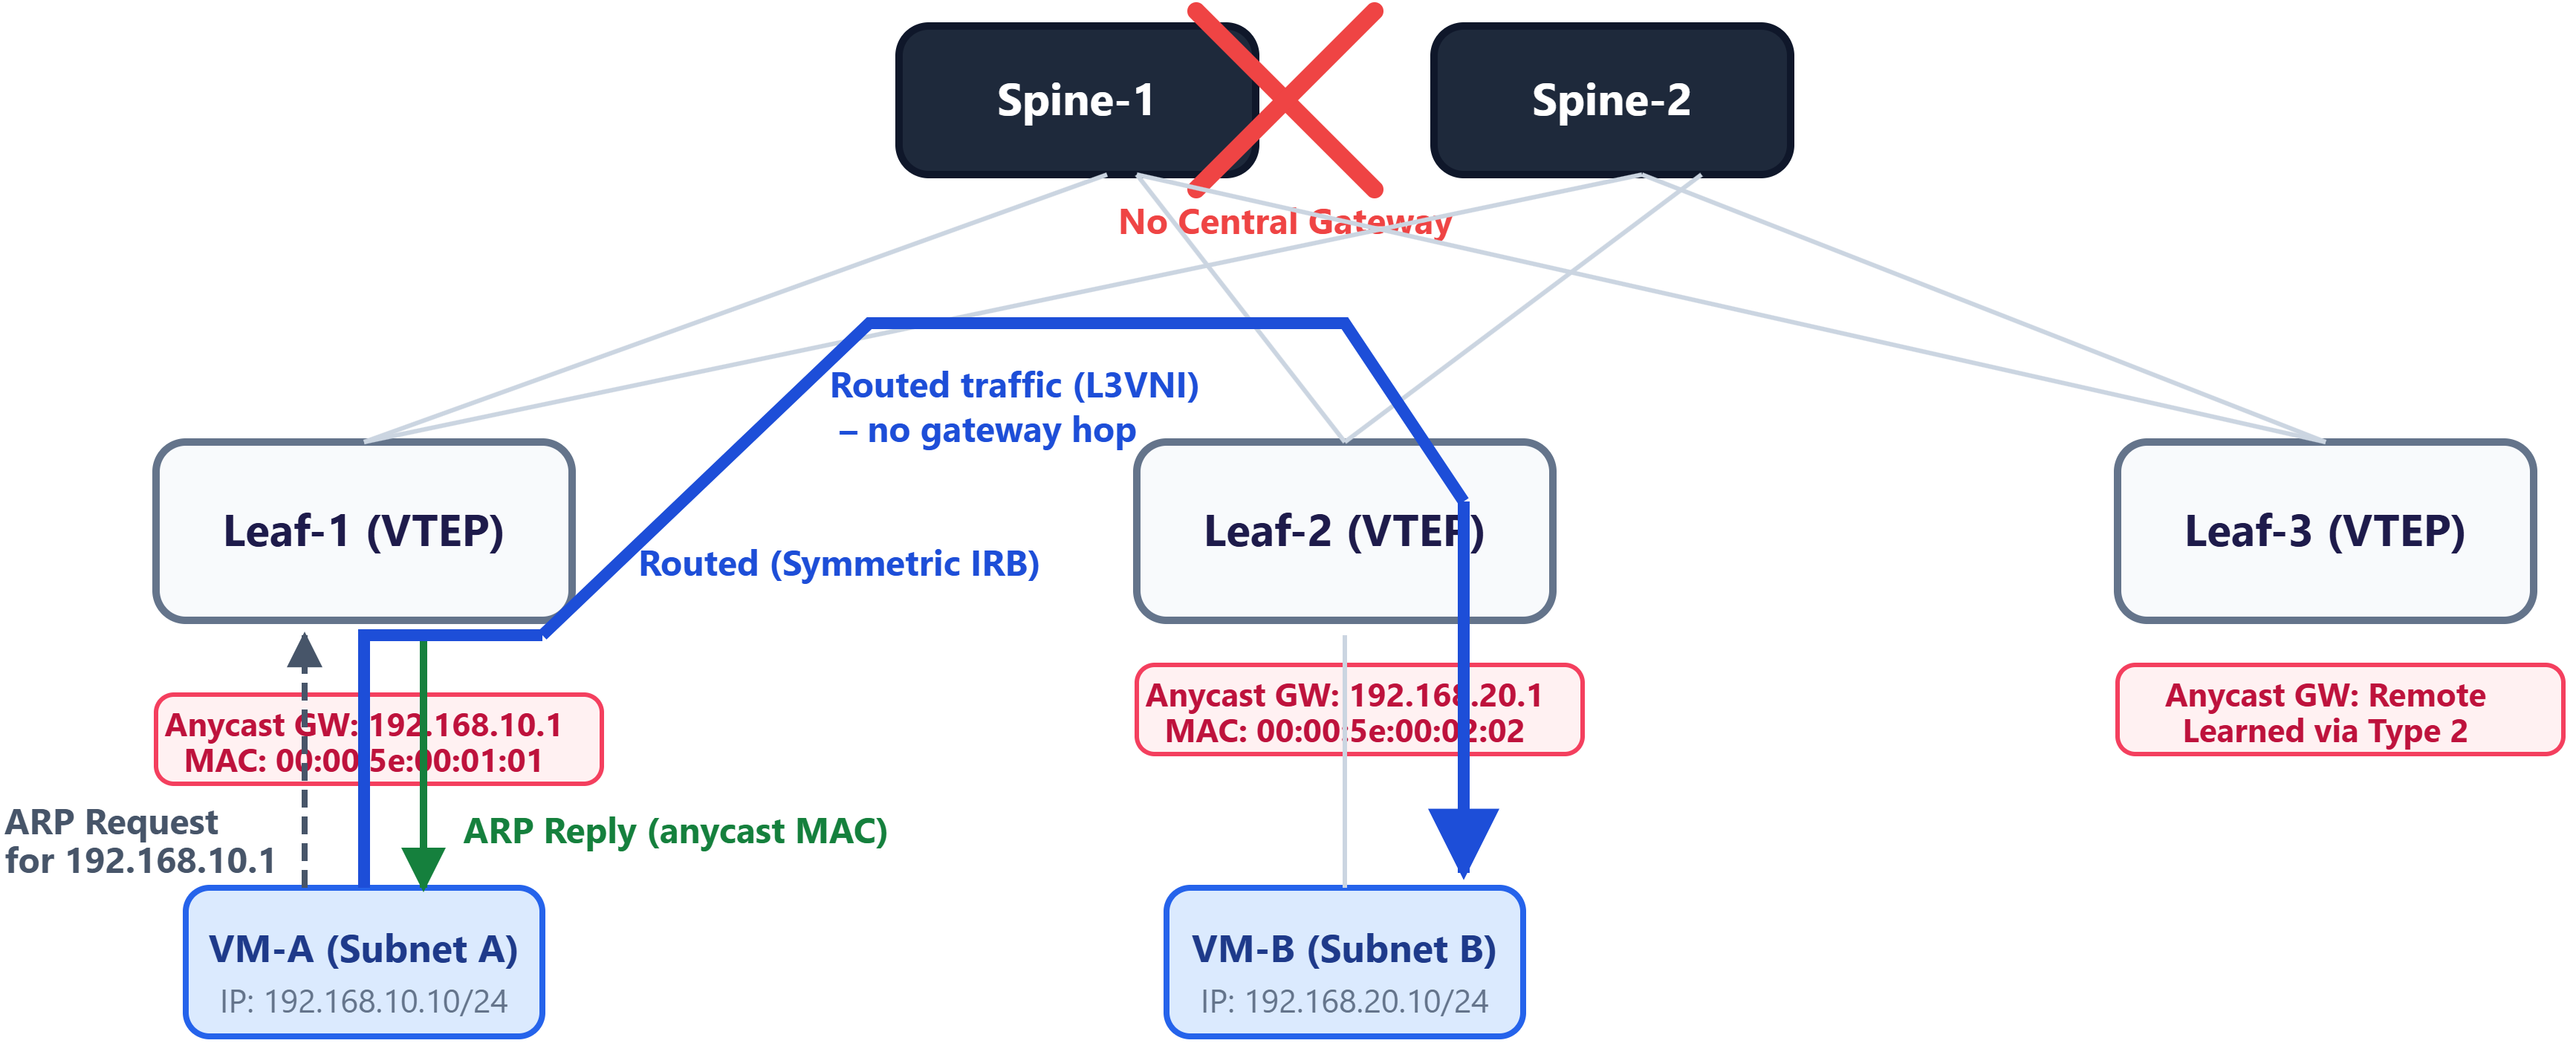
\includegraphics[width=\textwidth,height=8cm]{Images/AnycastGateway.png}}
\newcommand{\automationtools}{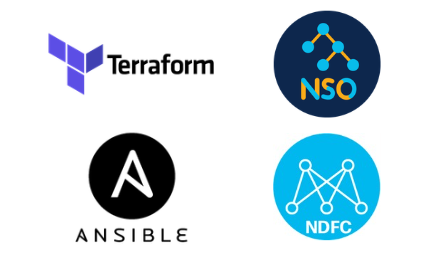
\includegraphics[width=\textwidth,height=5cm]{Images/Tools_logo.png}}
\newcommand{\ArchitectureTopology}{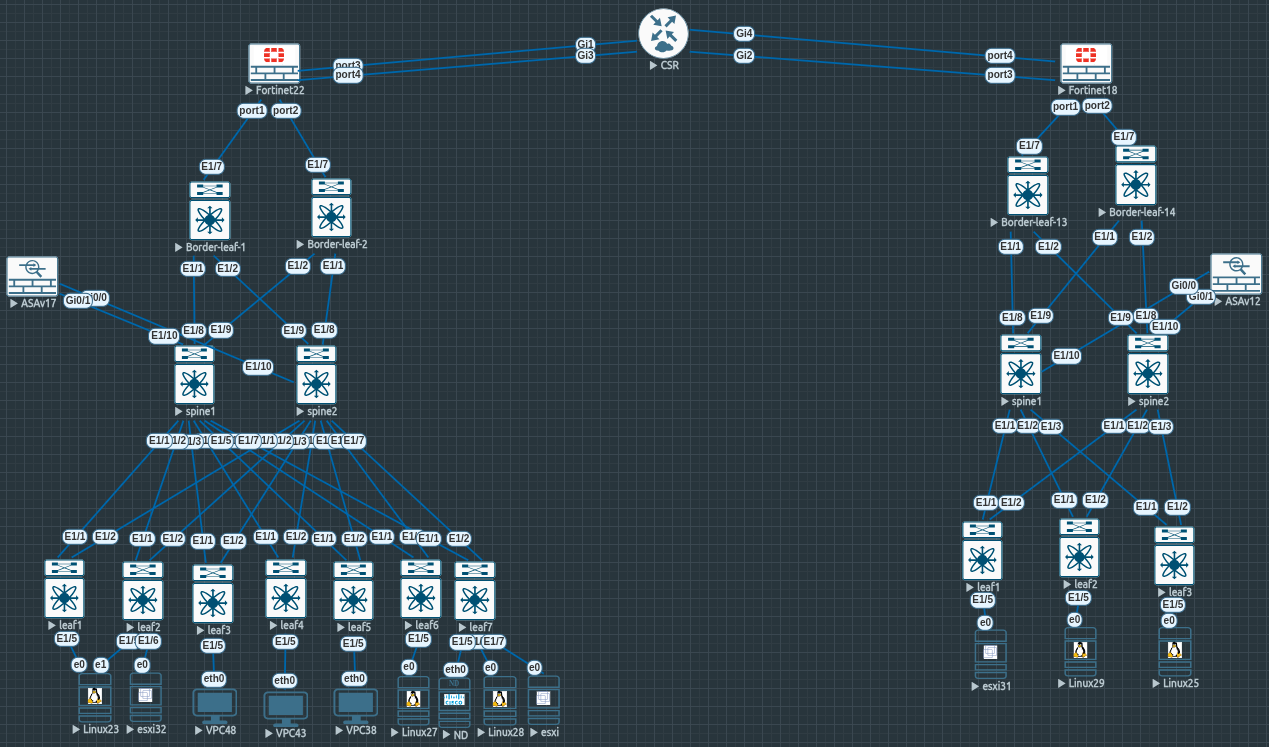
\includegraphics[width=\textwidth,height=8.5cm]{Images/Archtopology.png}}



%screenshots
\newcommand{\OspfRouting}{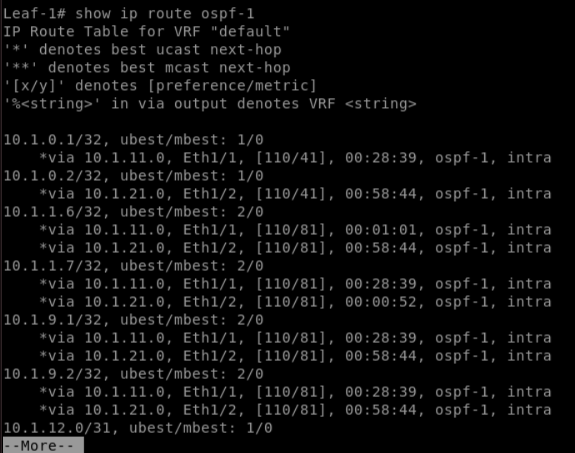
\includegraphics[width=\textwidth,height=6.6cm]{Images/Ospfrouting.png}}
\newcommand{\OspfSpine}{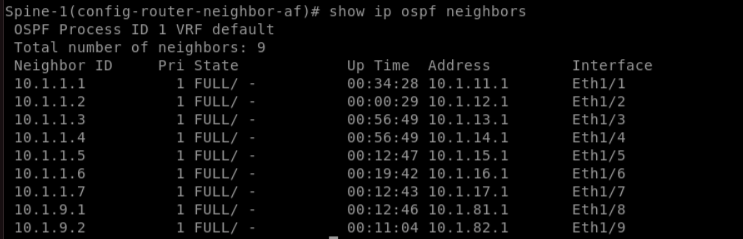
\includegraphics[width=\textwidth,height=7cm]{Images/OspfSpine.png}}
\newcommand{\loopbackreachability}{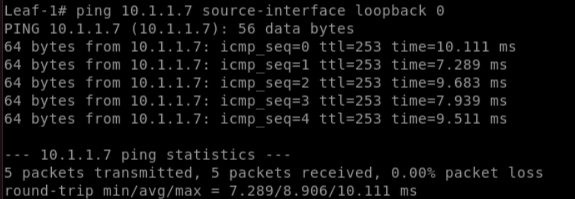
\includegraphics[width=\textwidth,height=3.9cm]{Images/Lobrechability.png}}
\newcommand{\EvpnLeaf}{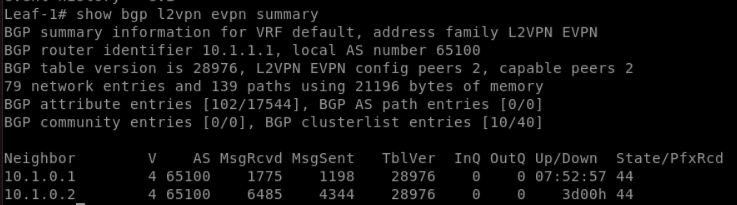
\includegraphics[width=\textwidth,height=3.5cm]{Images/overlayleaf.png}}
\newcommand{\nvepeers}{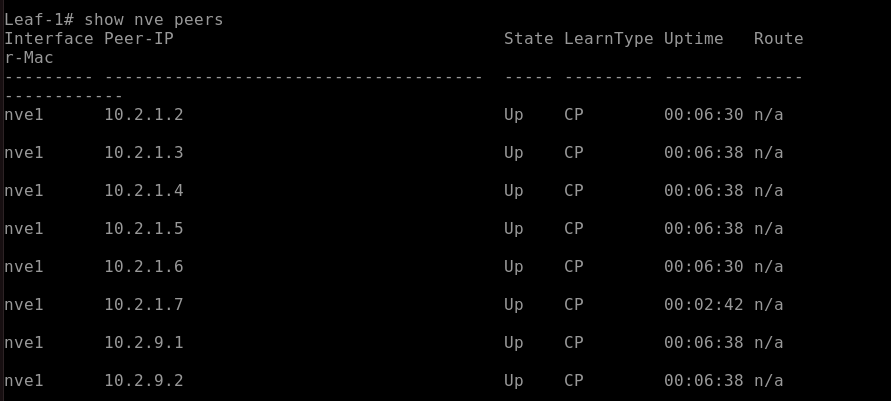
\includegraphics[width=\textwidth,height=4cm]{Images/NVETABLE.png}}
\newcommand{\EVPNroute}{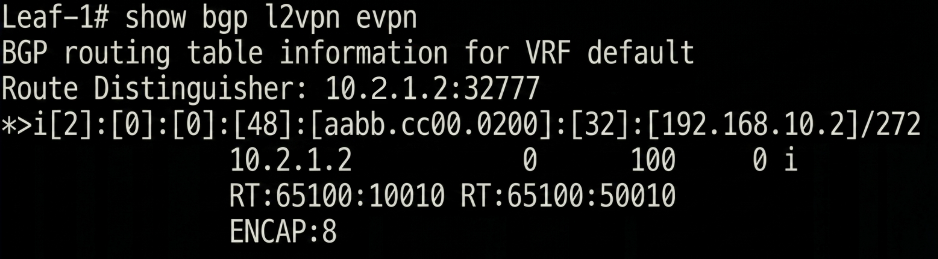
\includegraphics[width=\textwidth,height=3cm]{Images/Leaf-1EVPNroute.png}}
\newcommand{\ARPsuppression}{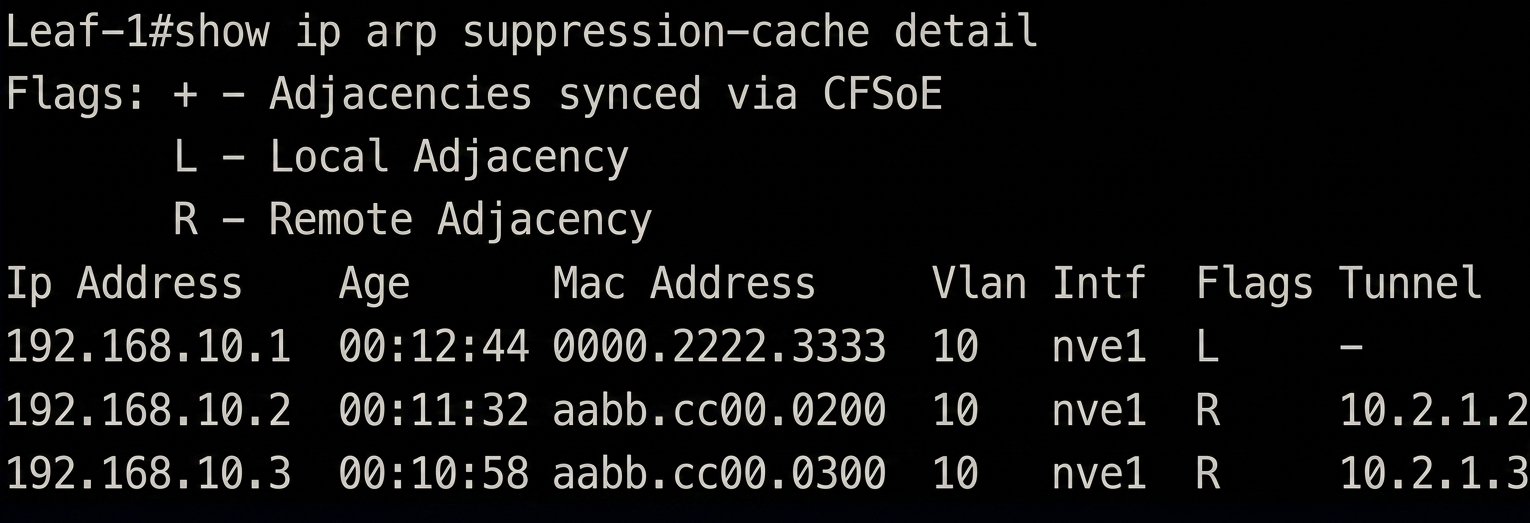
\includegraphics[width=\textwidth,height=3cm]{Images/ARPsuppressioncache.png}}
\newcommand{\BUMEVPNTRAFFIC}{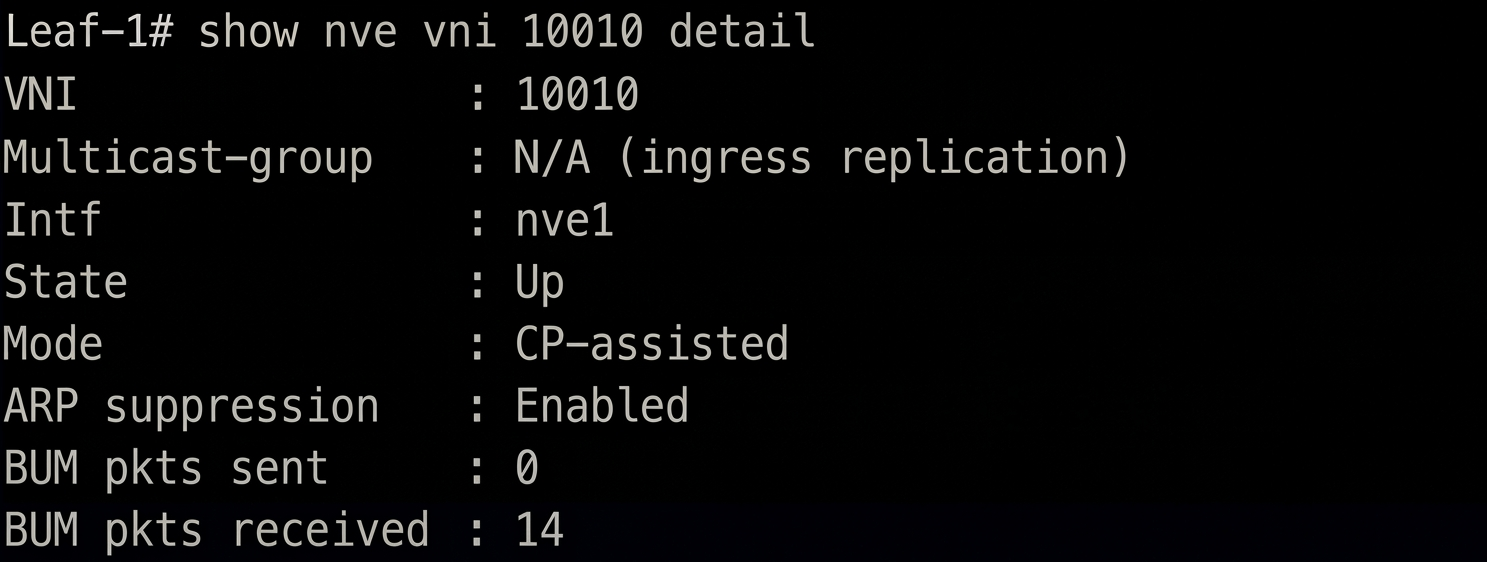
\includegraphics[width=\textwidth,height=3.5cm]{Images/NVEBUMtraffic.png}}
\newcommand{\beformigration}{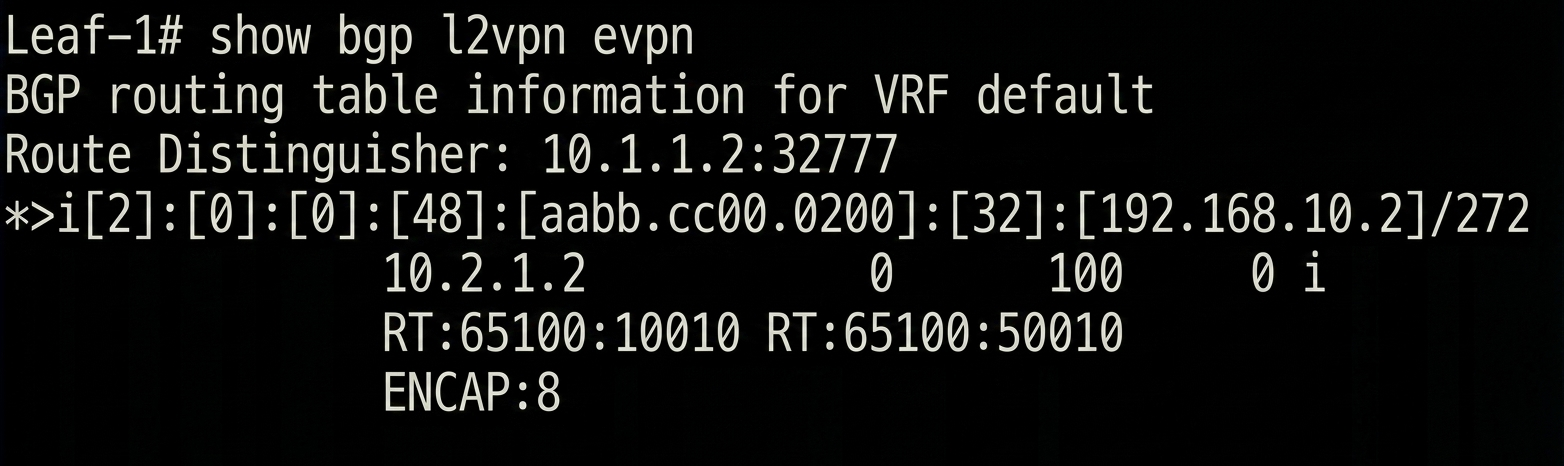
\includegraphics[width=\textwidth,height=3cm]{Images/EVPNroutebeforemigration.png}}
\newcommand{\aftermigration}{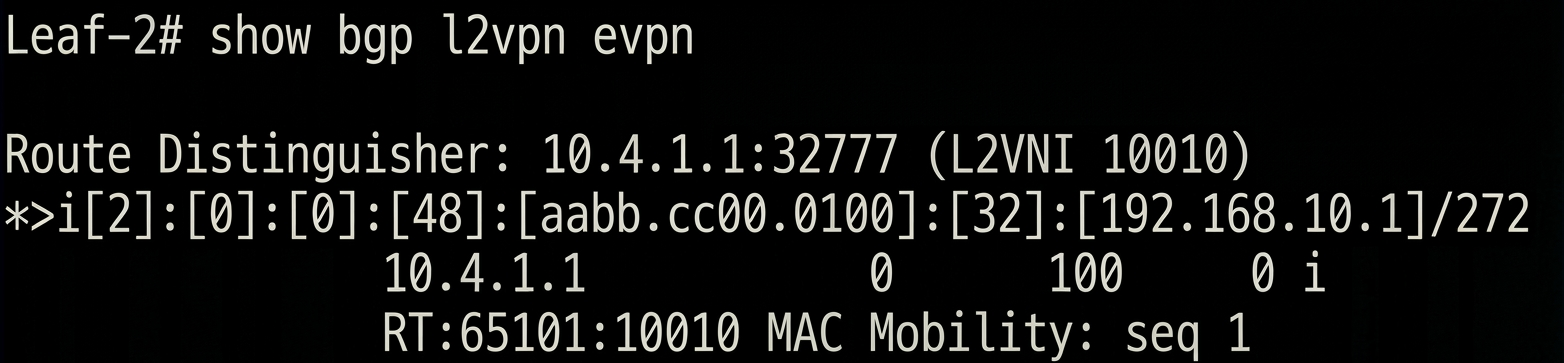
\includegraphics[width=\textwidth,height=3cm]{Images/EVPNrouteaftermigration.png}}
\newcommand{\forwardingdatabase}{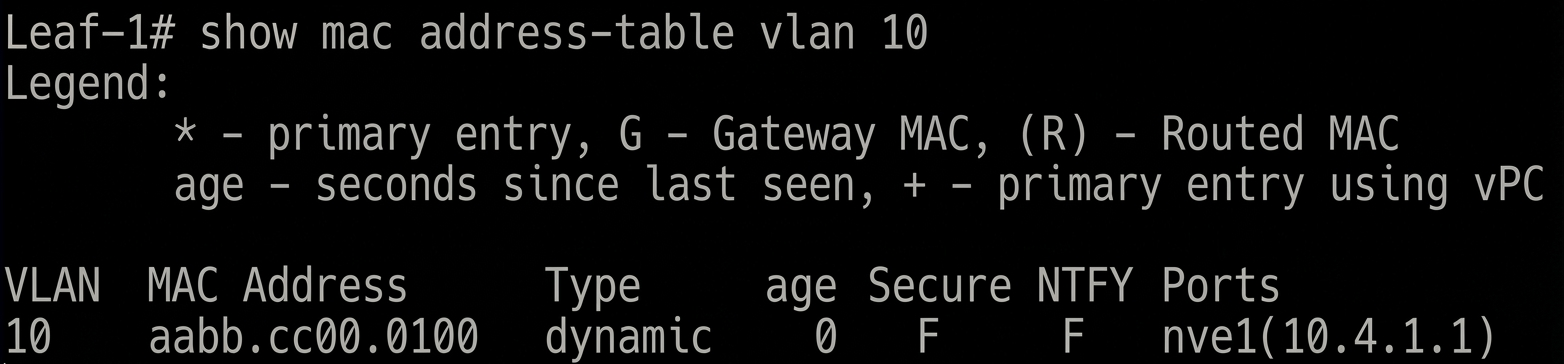
\includegraphics[width=\textwidth,height=3.5cm]{Images/forwardingdatabase.png}}
\newcommand{\crosssite}{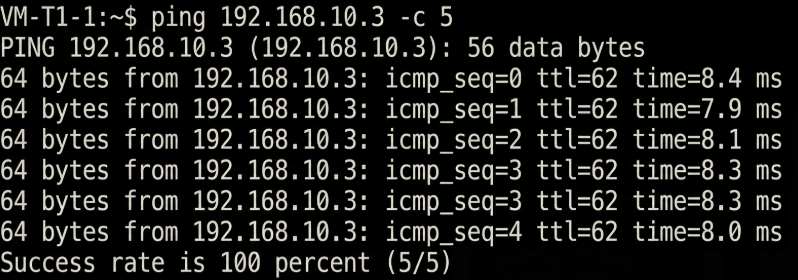
\includegraphics[width=\textwidth,height=3cm]{Images/Crosssiteping.png}}
\newcommand{\Typeroutes}{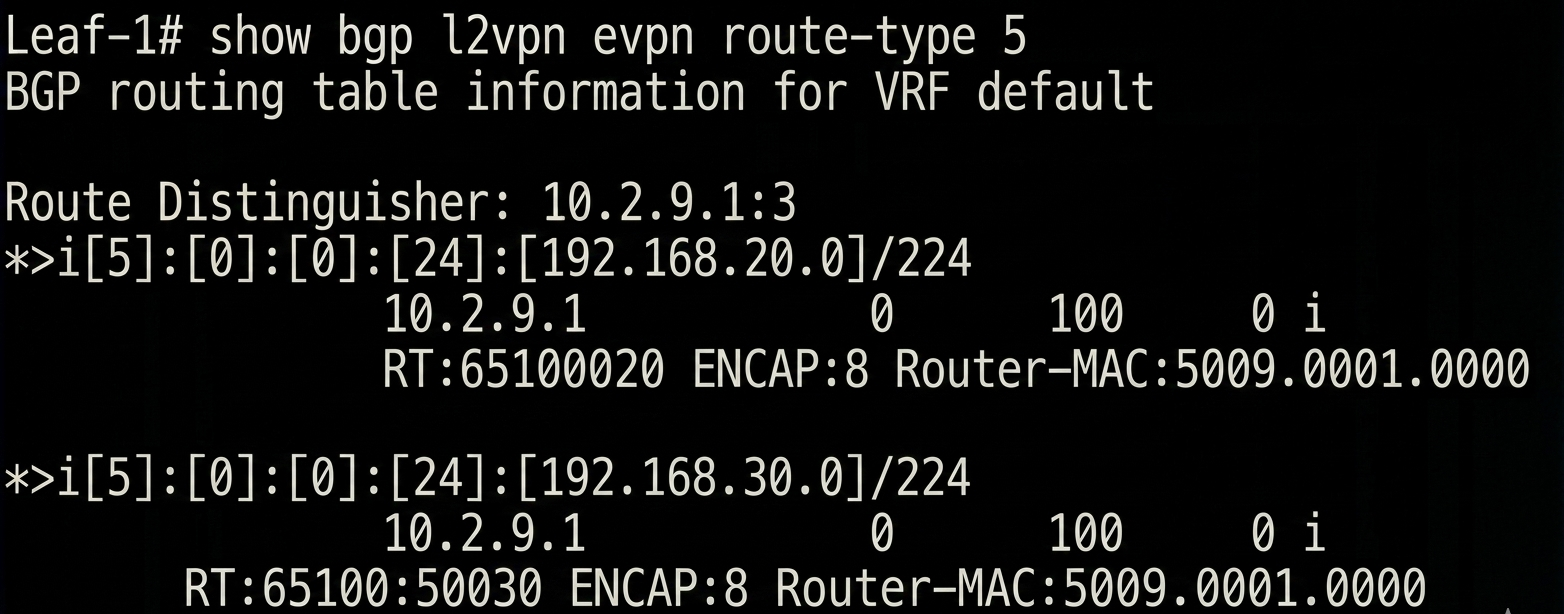
\includegraphics[width=\textwidth,height=3cm]{Images/Type5routes.png}}
\newcommand{\VRFrouting}{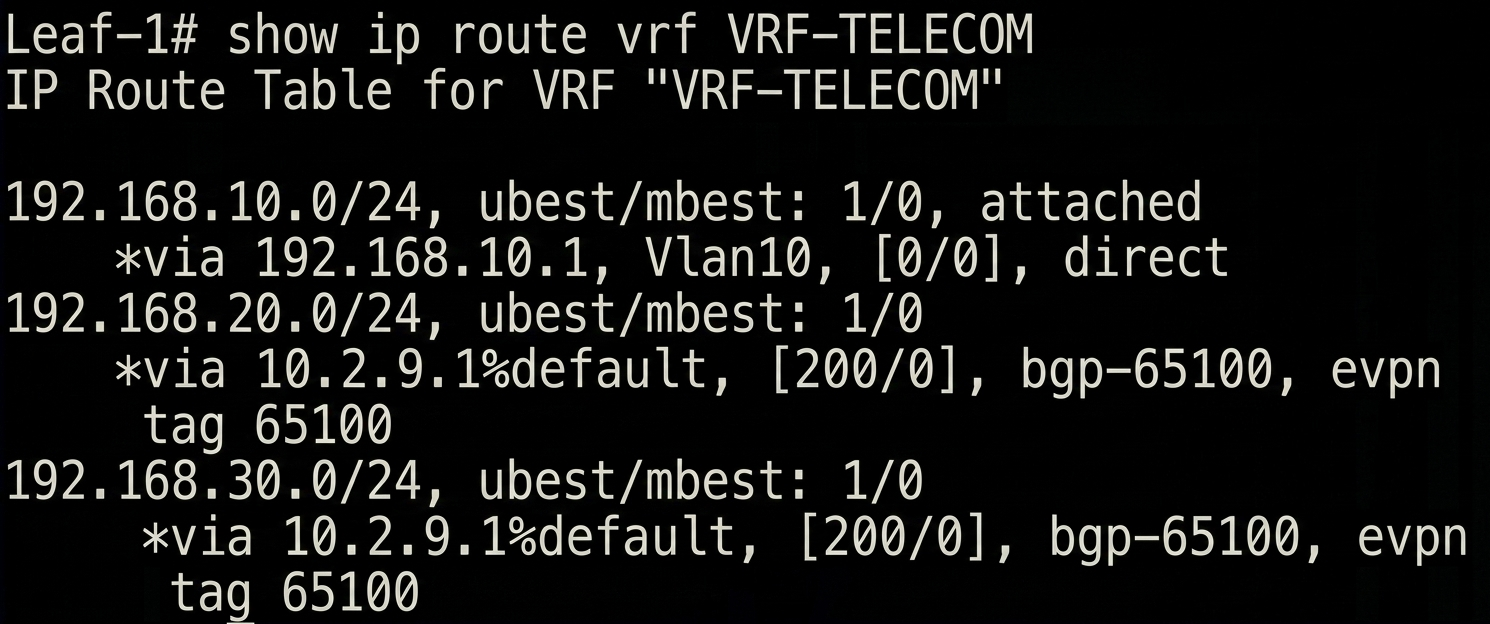
\includegraphics[width=\textwidth,height=3cm]{Images/VRFrouting.png}}
\newcommand{\intersite}{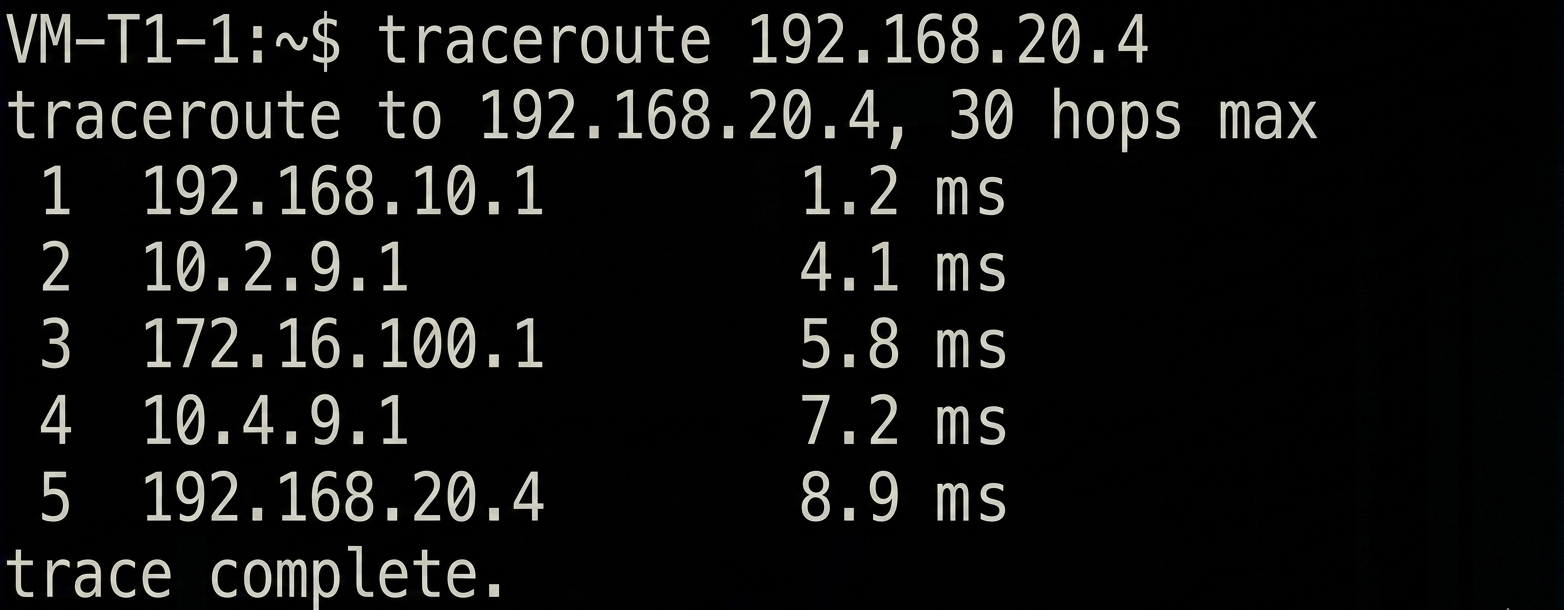
\includegraphics[width=\textwidth,height=3cm]{Images/Intersitetrace.png}}
\newcommand{\pahesI}{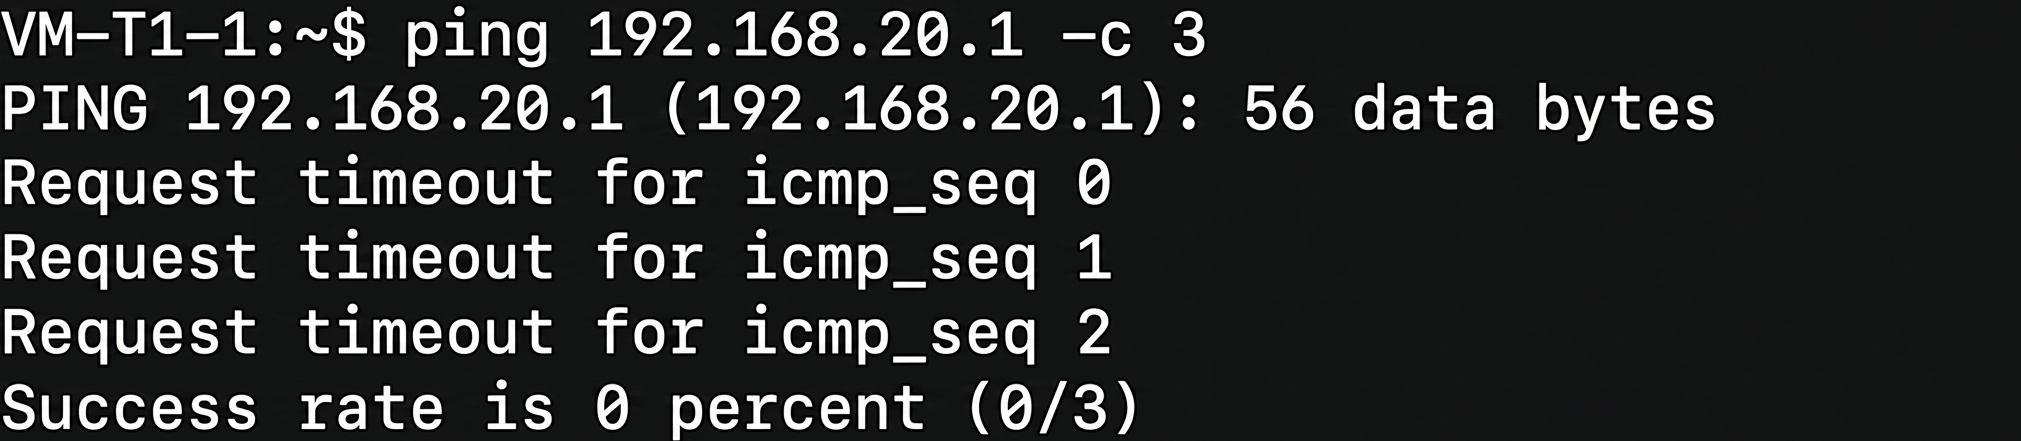
\includegraphics[width=\textwidth,height=3cm]{Images/VRFroutingtablePhaseI.png}}
\newcommand{\phaseII}{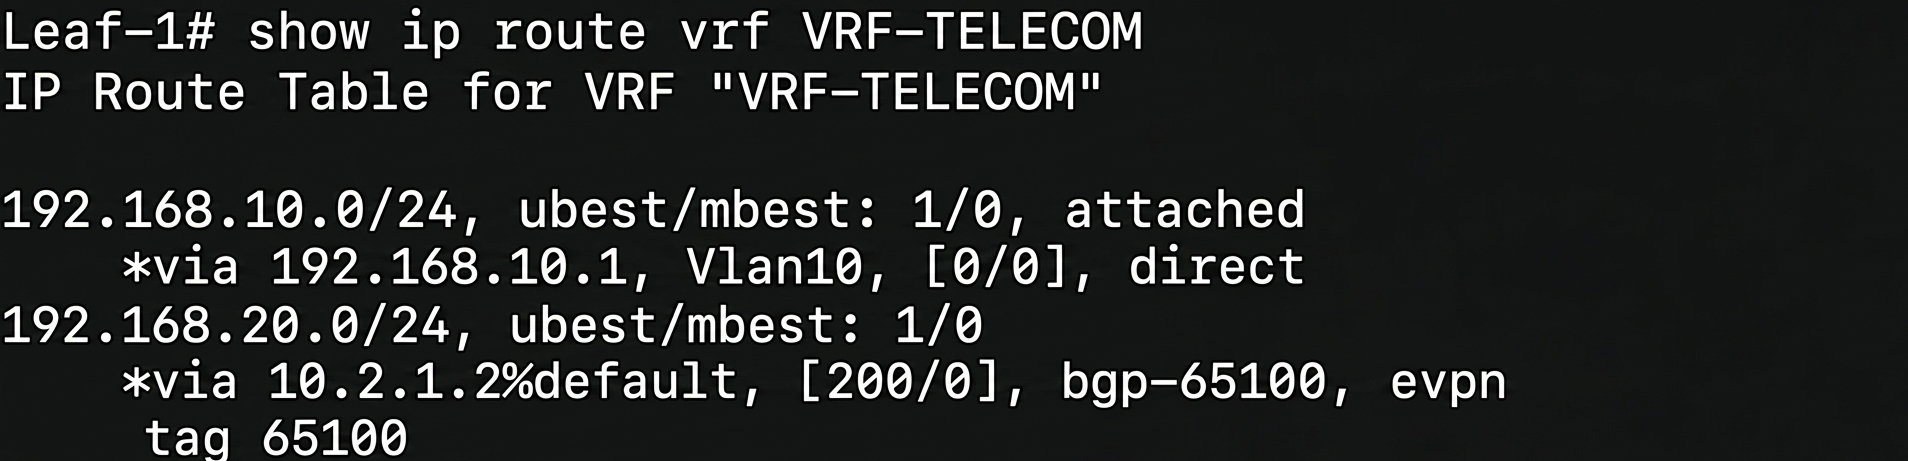
\includegraphics[width=\textwidth,height=3cm]{Images/VRFroutingtablePhaseII.png}}
\newcommand{\corsstenat}{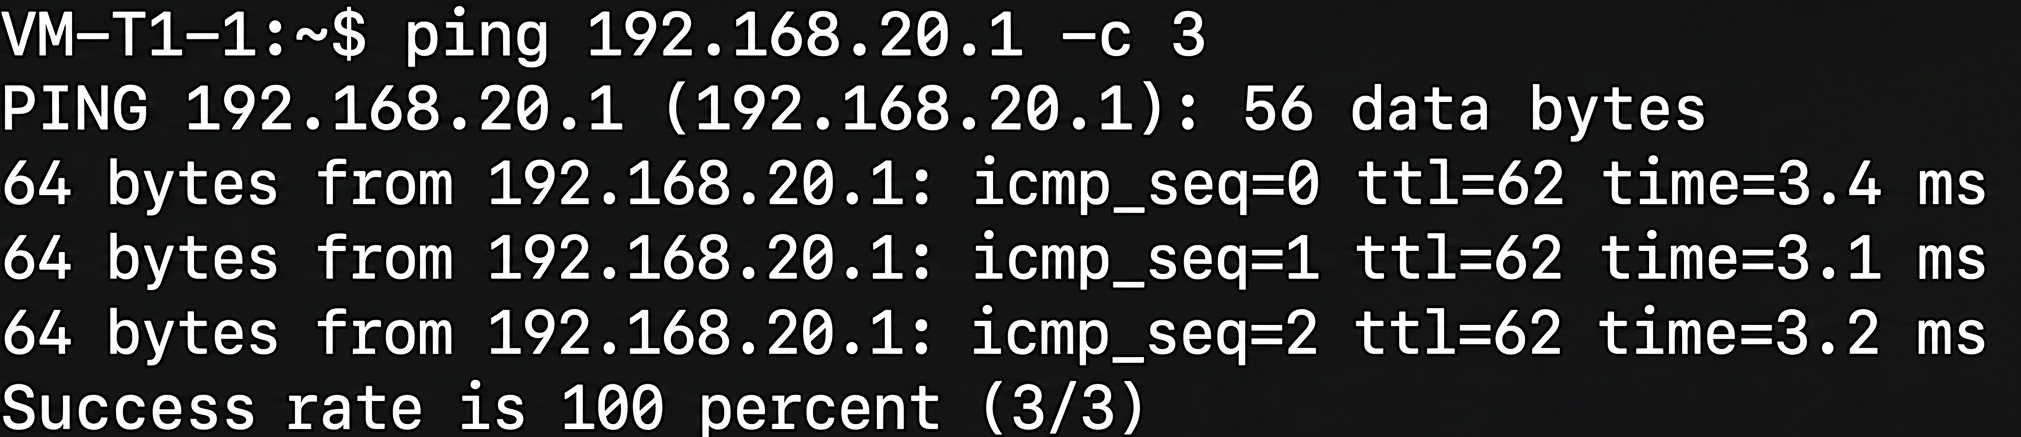
\includegraphics[width=\textwidth,height=3cm]{Images/PhaseCross-tenantpingsuccessafterrouteleak.png}}
\newcommand{\corsstenatfa}{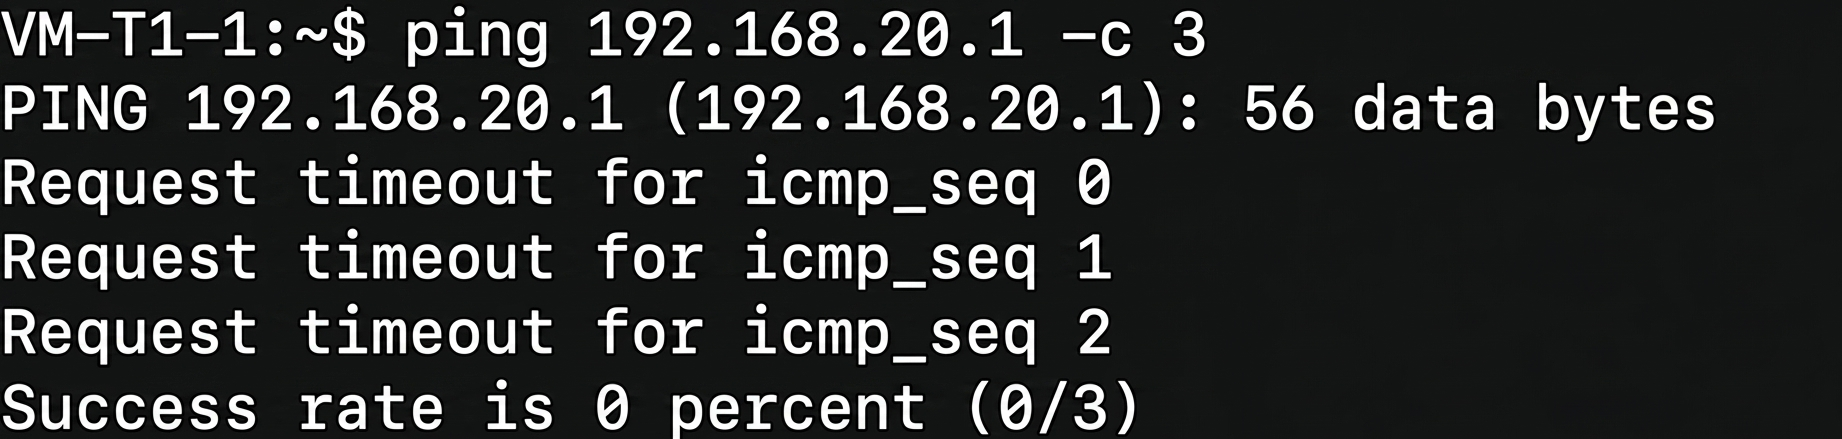
\includegraphics[width=\textwidth,height=3cm]{Images/Coss-tenantpingfailure.png}}
\newcommand{\VRFCLIENT}{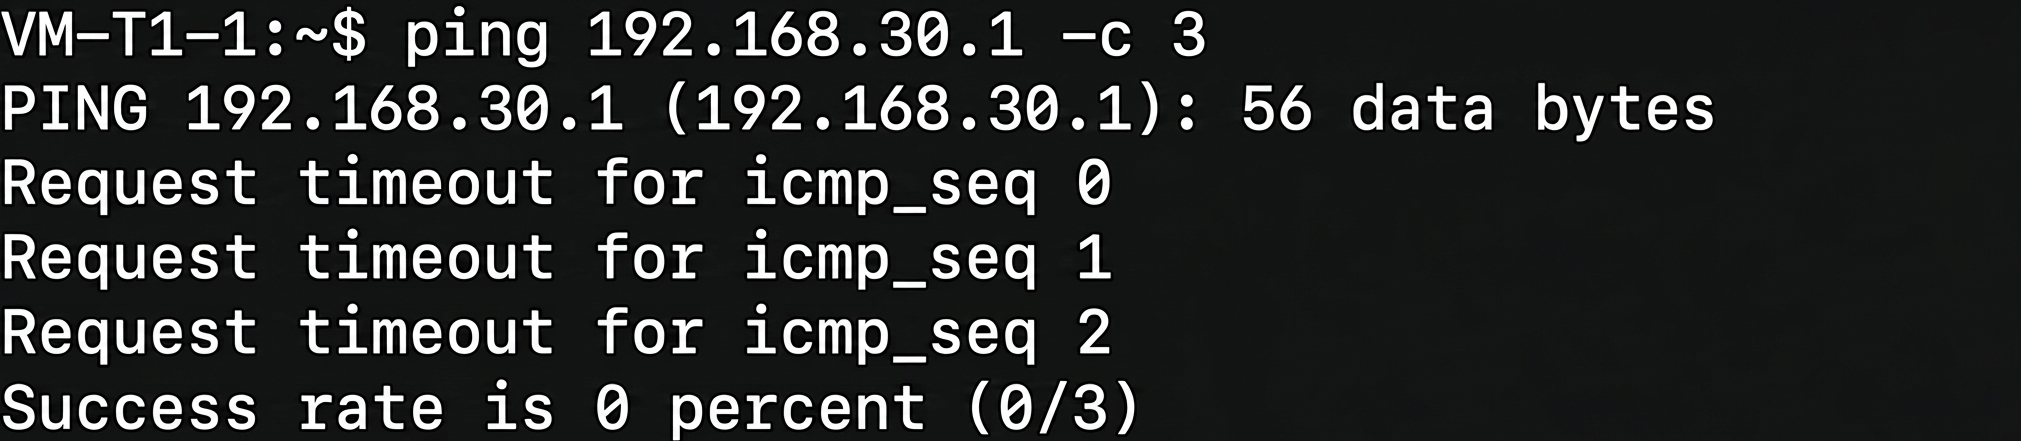
\includegraphics[width=\textwidth,height=3cm]{Images/VRF-CLIENTisolation.png}}
\newcommand{\bfdsucc}{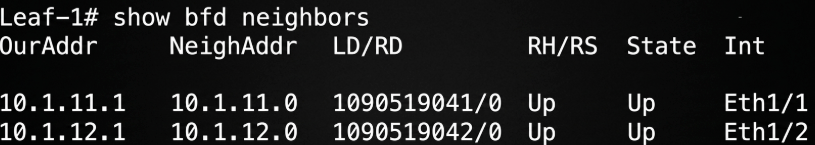
\includegraphics[width=\textwidth,height=3cm]{Images/BFDneighborsucc.png}}
\newcommand{\bfdfail}{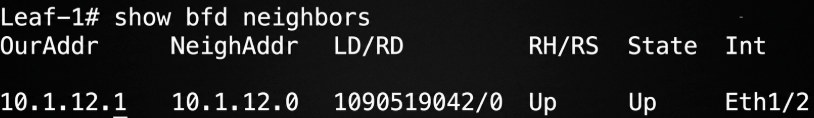
\includegraphics[width=\textwidth,height=3cm]{Images/BFDneighborfail.png}}
\newcommand{\Ipsec}{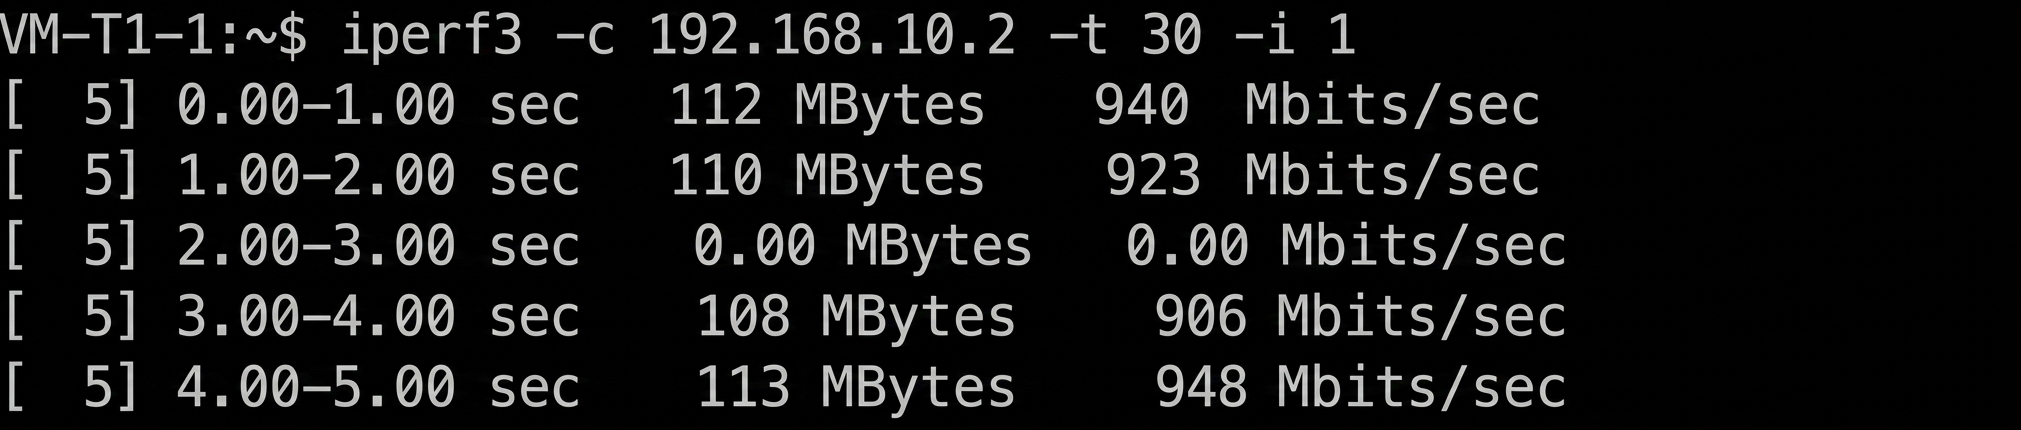
\includegraphics[width=\textwidth,height=3cm]{Images/iperf3traffic.png}}
\newcommand{\Ospfleaf}{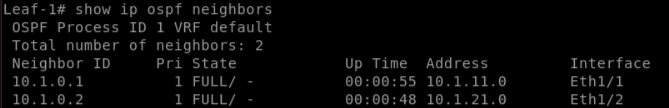
\includegraphics[width=\textwidth,height=3cm]{Images/OspfLeaf.png}}
\newcommand{\Ospfleaffailer}{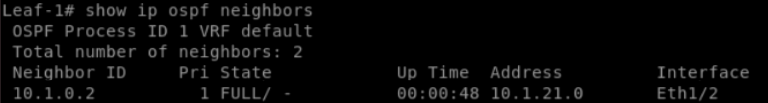
\includegraphics[width=\textwidth,height=3cm]{Images/ospfleaffailer.png}}
\newcommand{\fabric}{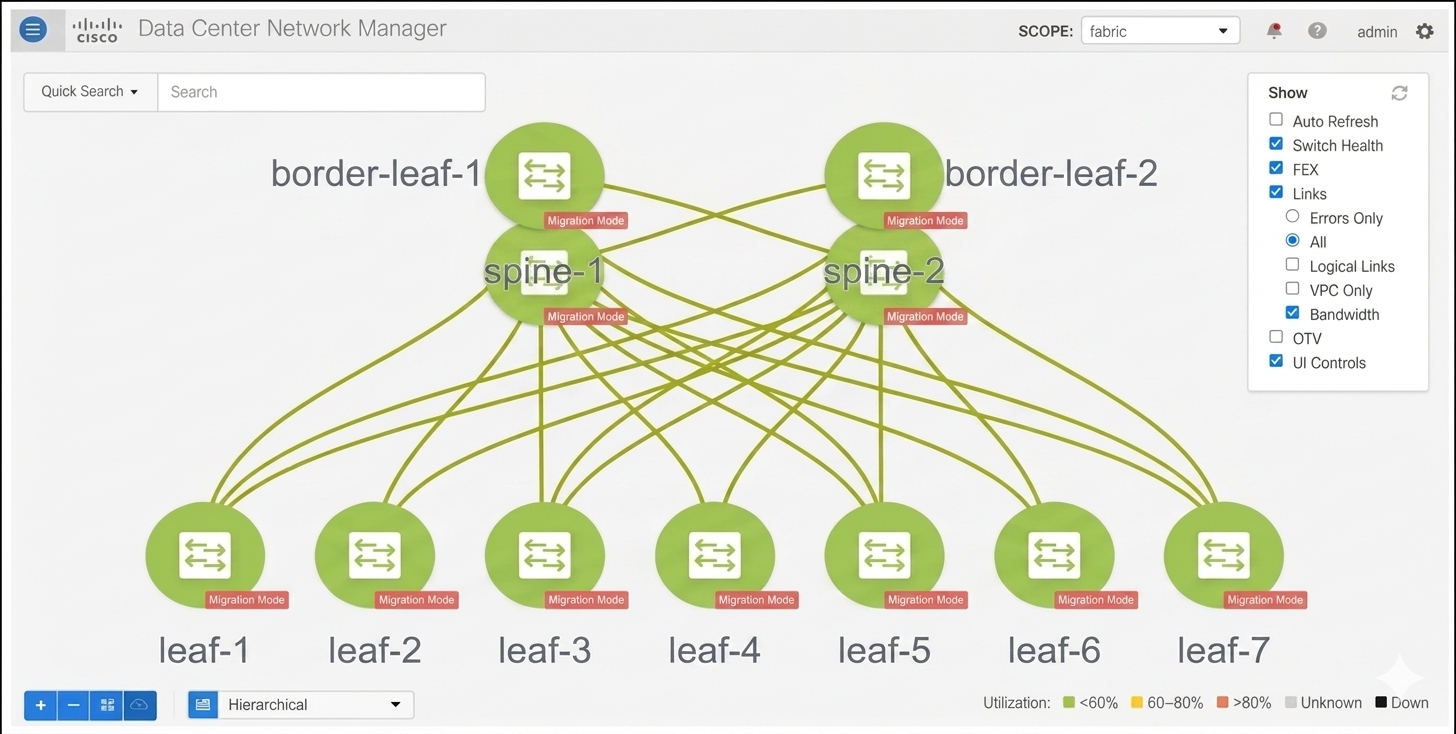
\includegraphics[width=\textwidth,height=6cm]{Images/fabriccontroller.png}}
\newcommand{\fabricdash}{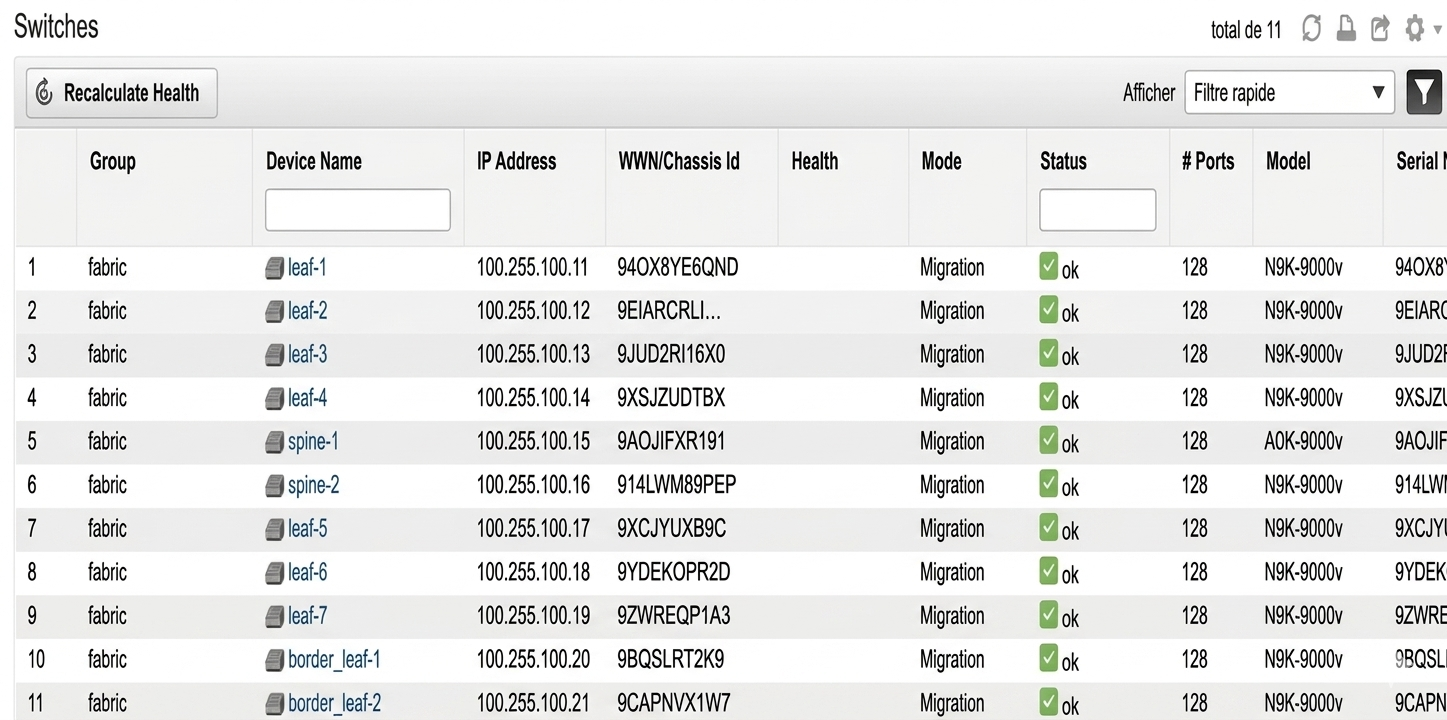
\includegraphics[width=\textwidth,height=6cm]{Images/dashbord.png}}


\newcolumntype{Y}{>{\raggedright\arraybackslash}X}
% No dots for chapters (common in theses/reports)
\renewcommand{\cftsecleader}{\cftdotfill{\cftdotsep}}   % add dots
\renewcommand{\cftsubsecleader}{\cftdotfill{\cftdotsep}}     % just in case
\renewcommand{\contentsname}{Table of Contents}
% Dots for sections and subsections (grey, spaced nicely)
\renewcommand{\cftsecleader}{\cftdotfill{\cftdotsep}}   % add dots
\renewcommand{\cftsubsecleader}{\cftdotfill{\cftdotsep}}

% Make dots grey (adjust 0.6 = medium grey; 0.4 = lighter)
\renewcommand{\cftdot}{\textcolor{gray!60}{\textperiodcentered}}  % grey dots

\titleformat{\section}
  {\normalfont\Large\bfseries\raggedright}
  {\thesection\enspace}
  {0pt}
  {}
\titlespacing*{\section}{0pt}{20pt}{10pt}

\titleformat{\subsection}
  {\normalfont\large\bfseries\raggedright}
  {\thesubsection\enspace}
  {0pt}
  {}
\titlespacing*{\subsection}{0pt}{15pt}{8pt}
\titlespacing*{\subsubsection}{0pt}{15pt}{8pt}


% Define colors FIRST
\definecolor{nexusblue}{RGB}{0, 112, 192}
\definecolor{nexusgray}{RGB}{128, 128, 128}
\definecolor{nexusgreen}{RGB}{0, 176, 80}
\definecolor{nexusorange}{RGB}{255, 153, 0}
\definecolor{nexusred}{RGB}{255, 0, 0}
\definecolor{background}{RGB}{245, 245, 245}
\definecolor{codeframe}{RGB}{200, 200, 200}

% Custom lst style for Cisco NX-OS
\lstdefinestyle{nexus}{
    language=bash,
    basicstyle=\ttfamily\footnotesize\color{black},
    backgroundcolor=\color{background},
    frame=single,
    rulecolor=\color{codeframe},
    frameround=tttt,
    framesep=5pt,
    xleftmargin=15pt,
    xrightmargin=10pt,
    aboveskip=10pt,
    belowskip=10pt,
    keywordstyle=[1]{\color{nexusblue}\bfseries},
    keywordstyle=[2]{\color{nexusgreen}\bfseries},
    keywordstyle=[3]{\color{nexusorange}\bfseries},
    commentstyle=\color{nexusgray}\itshape,
    stringstyle=\color{nexusred},
    numbers=none,              % <-- REMOVED line numbers
    showstringspaces=false,
    breaklines=true,
    breakatwhitespace=true,
    tabsize=2,
    captionpos=b,
    abovecaptionskip=10pt,
    belowcaptionskip=5pt,
    literate={-}{-}1
}

% Cisco NX-OS keywords
\lstset{
    style=nexus,
    morekeywords=[1]{
        feature, interface, no, shutdown, ip, router, ospf, bfd,
        mtu, description, vrf, context, member, address, family,
        unicast, route, target, both, auto, evpn, vni, vn, segment,
        vlan, fabric, forwarding, mode, anycast, gateway, mac,
        bgp, neighbor, remote, as, update, source, loopback,
        send, community, extended, route, reflector, client,
        retain, all, address, family, l2vpn, ebgp, multihop,
        peer, type, fabric, external, rewrite, rt, asn
    },
    morekeywords=[2]{
        Ethernet, loopback, Vlan, nve, GigabitEthernet
    },
    morekeywords=[3]{
        300, 9216, 0.0.0.0, 10.1.11.1, 31, 65001, 65101
    }
}
\usepackage[colorlinks=true,
            citecolor=blue,
            linkcolor=black,
            urlcolor=blue,
            pdfborder={0 0 0}]{hyperref}

% --- Body text full justification (LaTeX default) ---
% No \sloppy, no \raggedright for body.
% Just ensure titles are ragged-right (already done via \titleformat with \raggedright)

% Fine-tune hyphenation to avoid ugly breaks like fre-quent
\hyphenpenalty=1000      % discourage hyphenation (default 50)
\exhyphenpenalty=1000
\righthyphenmin=3        % minimum letters before hyphen (default 3)
\lefthyphenmin=3         % minimum letters after hyphen (default 2)

% Prevent specific bad hyphenations
\hyphenation{frequent}
\hyphenation{architecture}
\hyphenation{protocol}
\hyphenation{encapsulation}